\documentclass{article}


% % if you need to pass options to natbib, use, e.g.:
%     \PassOptionsToPackage{numbers, compress}{natbib}
% % before loading neurips_2023


% % ready for submission
% % \usepackage{neurips_2023}
% \usepackage[final]{neurips_2024}


% % to compile a preprint version, e.g., for submission to arXiv, add add the
% % [preprint] option:
%     % \usepackage[preprint]{neurips_2023}


% % to compile a camera-ready version, add the [final] option, e.g.:
% %     \usepackage[final]{neurips_2023}

% % \usepackage[final]{neurips_2023}

% % to avoid loading the natbib package, add option nonatbib:
% %    \usepackage[nonatbib]{neurips_2023}

% \usepackage[utf8]{inputenc} % allow utf-8 input
% \usepackage[T1]{fontenc}    % use 8-bit T1 fonts
% \usepackage{hyperref}       % hyperlinks
% \usepackage{url}            % simple URL typesetting
% \usepackage{booktabs}       % professional-quality tables
% \usepackage{amsfonts}       % blackboard math symbols
% \usepackage{nicefrac}       % compact symbols for 1/2, etc.
% \usepackage{microtype}      % microtypography
% \usepackage{xcolor}         % colors
% \usepackage{multirow}
% \usepackage{amsmath}
% \usepackage[ruled]{algorithm2e} % Required for the algorithm environment
% \usepackage{graphicx} % Required for inserting images
% \usepackage{tcolorbox}
% \usepackage{caption}
% \usepackage{menukeys}
% \usepackage{amsthm}
% % \usepackage[margin=1in]{geometry} % Adjust margins to ensure the table fits well
% \usepackage{tabularx} % Import tabularx for tables that can adjust their width automaticallyu
% % \usepackage{wraptable}
% \usepackage{wrapfig,lipsum,booktabs}
% \usepackage{enumitem}

% % \usepackage{algorithm}
% % \usepackage{algpseudocode}

% \usepackage{array}
% \usepackage{amssymb}

% \newcolumntype{M}[1]{>{\centering\arraybackslash}p{#1}}


% \newcommand{\model}[0]{\textsc{AlphaLLM}}
% \newcommand{\emcts}[0]{$\eta$\textsc{Mcts}}
% \newcommand{\prm}[0]{\texttt{PRM}}
% \newcommand{\orm}[0]{\texttt{ORM}}

% \newcommand{\ie}[0]{\emph{i.e., }}
% \newcommand{\ea}[0]{\emph{et al. }}
% \newcommand{\eg}[0]{\emph{e.g., }}
% \newcommand{\cf}[0]{\emph{cf. }}
% \newcommand{\etc}[0]{\emph{etc.}}
% \newcommand{\aka}[0]{\emph{a.k.a. }}
% \newcommand{\RN}[1]{%
% 	\textup{\lowercase\expandafter{\it \romannumeral#1}}%
% }
% \newcommand{\enterkey}[0]{{\scriptsize{\keys{\return}}}}

% %%%%% NEW MATH DEFINITIONS %%%%%

\usepackage{amsmath,amsfonts,bm}

% Mark sections of captions for referring to divisions of figures
\newcommand{\figleft}{{\em (Left)}}
\newcommand{\figcenter}{{\em (Center)}}
\newcommand{\figright}{{\em (Right)}}
\newcommand{\figtop}{{\em (Top)}}
\newcommand{\figbottom}{{\em (Bottom)}}
\newcommand{\captiona}{{\em (a)}}
\newcommand{\captionb}{{\em (b)}}
\newcommand{\captionc}{{\em (c)}}
\newcommand{\captiond}{{\em (d)}}

% Highlight a newly defined term
\newcommand{\newterm}[1]{{\bf #1}}


% Figure reference, lower-case.
\def\figref#1{figure~\ref{#1}}
% Figure reference, capital. For start of sentence
\def\Figref#1{Figure~\ref{#1}}
\def\twofigref#1#2{figures \ref{#1} and \ref{#2}}
\def\quadfigref#1#2#3#4{figures \ref{#1}, \ref{#2}, \ref{#3} and \ref{#4}}
% Section reference, lower-case.
\def\secref#1{section~\ref{#1}}
% Section reference, capital.
\def\Secref#1{Section~\ref{#1}}
% Reference to two sections.
\def\twosecrefs#1#2{sections \ref{#1} and \ref{#2}}
% Reference to three sections.
\def\secrefs#1#2#3{sections \ref{#1}, \ref{#2} and \ref{#3}}
% Reference to an equation, lower-case.
\def\eqref#1{equation~\ref{#1}}
% Reference to an equation, upper case
\def\Eqref#1{Equation~\ref{#1}}
% A raw reference to an equation---avoid using if possible
\def\plaineqref#1{\ref{#1}}
% Reference to a chapter, lower-case.
\def\chapref#1{chapter~\ref{#1}}
% Reference to an equation, upper case.
\def\Chapref#1{Chapter~\ref{#1}}
% Reference to a range of chapters
\def\rangechapref#1#2{chapters\ref{#1}--\ref{#2}}
% Reference to an algorithm, lower-case.
\def\algref#1{algorithm~\ref{#1}}
% Reference to an algorithm, upper case.
\def\Algref#1{Algorithm~\ref{#1}}
\def\twoalgref#1#2{algorithms \ref{#1} and \ref{#2}}
\def\Twoalgref#1#2{Algorithms \ref{#1} and \ref{#2}}
% Reference to a part, lower case
\def\partref#1{part~\ref{#1}}
% Reference to a part, upper case
\def\Partref#1{Part~\ref{#1}}
\def\twopartref#1#2{parts \ref{#1} and \ref{#2}}

\def\ceil#1{\lceil #1 \rceil}
\def\floor#1{\lfloor #1 \rfloor}
\def\1{\bm{1}}
\newcommand{\train}{\mathcal{D}}
\newcommand{\valid}{\mathcal{D_{\mathrm{valid}}}}
\newcommand{\test}{\mathcal{D_{\mathrm{test}}}}

\def\eps{{\epsilon}}


% Random variables
\def\reta{{\textnormal{$\eta$}}}
\def\ra{{\textnormal{a}}}
\def\rb{{\textnormal{b}}}
\def\rc{{\textnormal{c}}}
\def\rd{{\textnormal{d}}}
\def\re{{\textnormal{e}}}
\def\rf{{\textnormal{f}}}
\def\rg{{\textnormal{g}}}
\def\rh{{\textnormal{h}}}
\def\ri{{\textnormal{i}}}
\def\rj{{\textnormal{j}}}
\def\rk{{\textnormal{k}}}
\def\rl{{\textnormal{l}}}
% rm is already a command, just don't name any random variables m
\def\rn{{\textnormal{n}}}
\def\ro{{\textnormal{o}}}
\def\rp{{\textnormal{p}}}
\def\rq{{\textnormal{q}}}
\def\rr{{\textnormal{r}}}
\def\rs{{\textnormal{s}}}
\def\rt{{\textnormal{t}}}
\def\ru{{\textnormal{u}}}
\def\rv{{\textnormal{v}}}
\def\rw{{\textnormal{w}}}
\def\rx{{\textnormal{x}}}
\def\ry{{\textnormal{y}}}
\def\rz{{\textnormal{z}}}

% Random vectors
\def\rvepsilon{{\mathbf{\epsilon}}}
\def\rvtheta{{\mathbf{\theta}}}
\def\rva{{\mathbf{a}}}
\def\rvb{{\mathbf{b}}}
\def\rvc{{\mathbf{c}}}
\def\rvd{{\mathbf{d}}}
\def\rve{{\mathbf{e}}}
\def\rvf{{\mathbf{f}}}
\def\rvg{{\mathbf{g}}}
\def\rvh{{\mathbf{h}}}
\def\rvu{{\mathbf{i}}}
\def\rvj{{\mathbf{j}}}
\def\rvk{{\mathbf{k}}}
\def\rvl{{\mathbf{l}}}
\def\rvm{{\mathbf{m}}}
\def\rvn{{\mathbf{n}}}
\def\rvo{{\mathbf{o}}}
\def\rvp{{\mathbf{p}}}
\def\rvq{{\mathbf{q}}}
\def\rvr{{\mathbf{r}}}
\def\rvs{{\mathbf{s}}}
\def\rvt{{\mathbf{t}}}
\def\rvu{{\mathbf{u}}}
\def\rvv{{\mathbf{v}}}
\def\rvw{{\mathbf{w}}}
\def\rvx{{\mathbf{x}}}
\def\rvy{{\mathbf{y}}}
\def\rvz{{\mathbf{z}}}

% Elements of random vectors
\def\erva{{\textnormal{a}}}
\def\ervb{{\textnormal{b}}}
\def\ervc{{\textnormal{c}}}
\def\ervd{{\textnormal{d}}}
\def\erve{{\textnormal{e}}}
\def\ervf{{\textnormal{f}}}
\def\ervg{{\textnormal{g}}}
\def\ervh{{\textnormal{h}}}
\def\ervi{{\textnormal{i}}}
\def\ervj{{\textnormal{j}}}
\def\ervk{{\textnormal{k}}}
\def\ervl{{\textnormal{l}}}
\def\ervm{{\textnormal{m}}}
\def\ervn{{\textnormal{n}}}
\def\ervo{{\textnormal{o}}}
\def\ervp{{\textnormal{p}}}
\def\ervq{{\textnormal{q}}}
\def\ervr{{\textnormal{r}}}
\def\ervs{{\textnormal{s}}}
\def\ervt{{\textnormal{t}}}
\def\ervu{{\textnormal{u}}}
\def\ervv{{\textnormal{v}}}
\def\ervw{{\textnormal{w}}}
\def\ervx{{\textnormal{x}}}
\def\ervy{{\textnormal{y}}}
\def\ervz{{\textnormal{z}}}

% Random matrices
\def\rmA{{\mathbf{A}}}
\def\rmB{{\mathbf{B}}}
\def\rmC{{\mathbf{C}}}
\def\rmD{{\mathbf{D}}}
\def\rmE{{\mathbf{E}}}
\def\rmF{{\mathbf{F}}}
\def\rmG{{\mathbf{G}}}
\def\rmH{{\mathbf{H}}}
\def\rmI{{\mathbf{I}}}
\def\rmJ{{\mathbf{J}}}
\def\rmK{{\mathbf{K}}}
\def\rmL{{\mathbf{L}}}
\def\rmM{{\mathbf{M}}}
\def\rmN{{\mathbf{N}}}
\def\rmO{{\mathbf{O}}}
\def\rmP{{\mathbf{P}}}
\def\rmQ{{\mathbf{Q}}}
\def\rmR{{\mathbf{R}}}
\def\rmS{{\mathbf{S}}}
\def\rmT{{\mathbf{T}}}
\def\rmU{{\mathbf{U}}}
\def\rmV{{\mathbf{V}}}
\def\rmW{{\mathbf{W}}}
\def\rmX{{\mathbf{X}}}
\def\rmY{{\mathbf{Y}}}
\def\rmZ{{\mathbf{Z}}}

% Elements of random matrices
\def\ermA{{\textnormal{A}}}
\def\ermB{{\textnormal{B}}}
\def\ermC{{\textnormal{C}}}
\def\ermD{{\textnormal{D}}}
\def\ermE{{\textnormal{E}}}
\def\ermF{{\textnormal{F}}}
\def\ermG{{\textnormal{G}}}
\def\ermH{{\textnormal{H}}}
\def\ermI{{\textnormal{I}}}
\def\ermJ{{\textnormal{J}}}
\def\ermK{{\textnormal{K}}}
\def\ermL{{\textnormal{L}}}
\def\ermM{{\textnormal{M}}}
\def\ermN{{\textnormal{N}}}
\def\ermO{{\textnormal{O}}}
\def\ermP{{\textnormal{P}}}
\def\ermQ{{\textnormal{Q}}}
\def\ermR{{\textnormal{R}}}
\def\ermS{{\textnormal{S}}}
\def\ermT{{\textnormal{T}}}
\def\ermU{{\textnormal{U}}}
\def\ermV{{\textnormal{V}}}
\def\ermW{{\textnormal{W}}}
\def\ermX{{\textnormal{X}}}
\def\ermY{{\textnormal{Y}}}
\def\ermZ{{\textnormal{Z}}}

% Vectors
\def\vzero{{\bm{0}}}
\def\vone{{\bm{1}}}
\def\vmu{{\bm{\mu}}}
\def\vtheta{{\bm{\theta}}}
\def\vtau{{\bm{\tau}}}
\def\va{{\bm{a}}}
\def\vb{{\bm{b}}}
\def\vc{{\bm{c}}}
\def\vd{{\bm{d}}}
\def\ve{{\bm{e}}}
\def\vf{{\bm{f}}}
\def\vg{{\bm{g}}}
\def\vh{{\bm{h}}}
\def\vi{{\bm{i}}}
\def\vj{{\bm{j}}}
\def\vk{{\bm{k}}}
\def\vl{{\bm{l}}}
\def\vm{{\bm{m}}}
\def\vn{{\bm{n}}}
\def\vo{{\bm{o}}}
\def\vp{{\bm{p}}}
\def\vq{{\bm{q}}}
\def\vr{{\bm{r}}}
\def\vs{{\bm{s}}}
\def\vt{{\bm{t}}}
\def\vu{{\bm{u}}}
\def\vv{{\bm{v}}}
\def\vw{{\bm{w}}}
\def\vx{{\bm{x}}}
\def\vy{{\bm{y}}}
\def\vz{{\bm{z}}}

% Elements of vectors
\def\evalpha{{\alpha}}
\def\evbeta{{\beta}}
\def\evepsilon{{\epsilon}}
\def\evlambda{{\lambda}}
\def\evomega{{\omega}}
\def\evmu{{\mu}}
\def\evpsi{{\psi}}
\def\evsigma{{\sigma}}
\def\evtheta{{\theta}}
\def\eva{{a}}
\def\evb{{b}}
\def\evc{{c}}
\def\evd{{d}}
\def\eve{{e}}
\def\evf{{f}}
\def\evg{{g}}
\def\evh{{h}}
\def\evi{{i}}
\def\evj{{j}}
\def\evk{{k}}
\def\evl{{l}}
\def\evm{{m}}
\def\evn{{n}}
\def\evo{{o}}
\def\evp{{p}}
\def\evq{{q}}
\def\evr{{r}}
\def\evs{{s}}
\def\evt{{t}}
\def\evu{{u}}
\def\evv{{v}}
\def\evw{{w}}
\def\evx{{x}}
\def\evy{{y}}
\def\evz{{z}}

% Matrix
\def\mA{{\bm{A}}}
\def\mB{{\bm{B}}}
\def\mC{{\bm{C}}}
\def\mD{{\bm{D}}}
\def\mE{{\bm{E}}}
\def\mF{{\bm{F}}}
\def\mG{{\bm{G}}}
\def\mH{{\bm{H}}}
\def\mI{{\bm{I}}}
\def\mJ{{\bm{J}}}
\def\mK{{\bm{K}}}
\def\mL{{\bm{L}}}
\def\mM{{\bm{M}}}
\def\mN{{\bm{N}}}
\def\mO{{\bm{O}}}
\def\mP{{\bm{P}}}
\def\mQ{{\bm{Q}}}
\def\mR{{\bm{R}}}
\def\mS{{\bm{S}}}
\def\mT{{\bm{T}}}
\def\mU{{\bm{U}}}
\def\mV{{\bm{V}}}
\def\mW{{\bm{W}}}
\def\mX{{\bm{X}}}
\def\mY{{\bm{Y}}}
\def\mZ{{\bm{Z}}}
\def\mBeta{{\bm{\beta}}}
\def\mPhi{{\bm{\Phi}}}
\def\mLambda{{\bm{\Lambda}}}
\def\mSigma{{\bm{\Sigma}}}

% Tensor
\DeclareMathAlphabet{\mathsfit}{\encodingdefault}{\sfdefault}{m}{sl}
\SetMathAlphabet{\mathsfit}{bold}{\encodingdefault}{\sfdefault}{bx}{n}
\newcommand{\tens}[1]{\bm{\mathsfit{#1}}}
\def\tA{{\tens{A}}}
\def\tB{{\tens{B}}}
\def\tC{{\tens{C}}}
\def\tD{{\tens{D}}}
\def\tE{{\tens{E}}}
\def\tF{{\tens{F}}}
\def\tG{{\tens{G}}}
\def\tH{{\tens{H}}}
\def\tI{{\tens{I}}}
\def\tJ{{\tens{J}}}
\def\tK{{\tens{K}}}
\def\tL{{\tens{L}}}
\def\tM{{\tens{M}}}
\def\tN{{\tens{N}}}
\def\tO{{\tens{O}}}
\def\tP{{\tens{P}}}
\def\tQ{{\tens{Q}}}
\def\tR{{\tens{R}}}
\def\tS{{\tens{S}}}
\def\tT{{\tens{T}}}
\def\tU{{\tens{U}}}
\def\tV{{\tens{V}}}
\def\tW{{\tens{W}}}
\def\tX{{\tens{X}}}
\def\tY{{\tens{Y}}}
\def\tZ{{\tens{Z}}}


% Graph
\def\gA{{\mathcal{A}}}
\def\gB{{\mathcal{B}}}
\def\gC{{\mathcal{C}}}
\def\gD{{\mathcal{D}}}
\def\gE{{\mathcal{E}}}
\def\gF{{\mathcal{F}}}
\def\gG{{\mathcal{G}}}
\def\gH{{\mathcal{H}}}
\def\gI{{\mathcal{I}}}
\def\gJ{{\mathcal{J}}}
\def\gK{{\mathcal{K}}}
\def\gL{{\mathcal{L}}}
\def\gM{{\mathcal{M}}}
\def\gN{{\mathcal{N}}}
\def\gO{{\mathcal{O}}}
\def\gP{{\mathcal{P}}}
\def\gQ{{\mathcal{Q}}}
\def\gR{{\mathcal{R}}}
\def\gS{{\mathcal{S}}}
\def\gT{{\mathcal{T}}}
\def\gU{{\mathcal{U}}}
\def\gV{{\mathcal{V}}}
\def\gW{{\mathcal{W}}}
\def\gX{{\mathcal{X}}}
\def\gY{{\mathcal{Y}}}
\def\gZ{{\mathcal{Z}}}

% Sets
\def\sA{{\mathbb{A}}}
\def\sB{{\mathbb{B}}}
\def\sC{{\mathbb{C}}}
\def\sD{{\mathbb{D}}}
% Don't use a set called E, because this would be the same as our symbol
% for expectation.
\def\sF{{\mathbb{F}}}
\def\sE{{\mathbb{E}}}
\def\sG{{\mathbb{G}}}
\def\sH{{\mathbb{H}}}
\def\sI{{\mathbb{I}}}
\def\sJ{{\mathbb{J}}}
\def\sK{{\mathbb{K}}}
\def\sL{{\mathbb{L}}}
\def\sM{{\mathbb{M}}}
\def\sN{{\mathbb{N}}}
\def\sO{{\mathbb{O}}}
\def\sP{{\mathbb{P}}}
\def\sQ{{\mathbb{Q}}}
\def\sR{{\mathbb{R}}}
\def\sS{{\mathbb{S}}}
\def\sT{{\mathbb{T}}}
\def\sU{{\mathbb{U}}}
\def\sV{{\mathbb{V}}}
\def\sW{{\mathbb{W}}}
\def\sX{{\mathbb{X}}}
\def\sY{{\mathbb{Y}}}
\def\sZ{{\mathbb{Z}}}

% Entries of a matrix
\def\emLambda{{\Lambda}}
\def\emA{{A}}
\def\emB{{B}}
\def\emC{{C}}
\def\emD{{D}}
\def\emE{{E}}
\def\emF{{F}}
\def\emG{{G}}
\def\emH{{H}}
\def\emI{{I}}
\def\emJ{{J}}
\def\emK{{K}}
\def\emL{{L}}
\def\emM{{M}}
\def\emN{{N}}
\def\emO{{O}}
\def\emP{{P}}
\def\emQ{{Q}}
\def\emR{{R}}
\def\emS{{S}}
\def\emT{{T}}
\def\emU{{U}}
\def\emV{{V}}
\def\emW{{W}}
\def\emX{{X}}
\def\emY{{Y}}
\def\emZ{{Z}}
\def\emSigma{{\Sigma}}

% entries of a tensor
% Same font as tensor, without \bm wrapper
\newcommand{\etens}[1]{\mathsfit{#1}}
\def\etLambda{{\etens{\Lambda}}}
\def\etA{{\etens{A}}}
\def\etB{{\etens{B}}}
\def\etC{{\etens{C}}}
\def\etD{{\etens{D}}}
\def\etE{{\etens{E}}}
\def\etF{{\etens{F}}}
\def\etG{{\etens{G}}}
\def\etH{{\etens{H}}}
\def\etI{{\etens{I}}}
\def\etJ{{\etens{J}}}
\def\etK{{\etens{K}}}
\def\etL{{\etens{L}}}
\def\etM{{\etens{M}}}
\def\etN{{\etens{N}}}
\def\etO{{\etens{O}}}
\def\etP{{\etens{P}}}
\def\etQ{{\etens{Q}}}
\def\etR{{\etens{R}}}
\def\etS{{\etens{S}}}
\def\etT{{\etens{T}}}
\def\etU{{\etens{U}}}
\def\etV{{\etens{V}}}
\def\etW{{\etens{W}}}
\def\etX{{\etens{X}}}
\def\etY{{\etens{Y}}}
\def\etZ{{\etens{Z}}}

% The true underlying data generating distribution
\newcommand{\pdata}{p_{\rm{data}}}
% The empirical distribution defined by the training set
\newcommand{\ptrain}{\hat{p}_{\rm{data}}}
\newcommand{\Ptrain}{\hat{P}_{\rm{data}}}
% The model distribution
\newcommand{\pmodel}{p_{\rm{model}}}
\newcommand{\Pmodel}{P_{\rm{model}}}
\newcommand{\ptildemodel}{\tilde{p}_{\rm{model}}}
% Stochastic autoencoder distributions
\newcommand{\pencode}{p_{\rm{encoder}}}
\newcommand{\pdecode}{p_{\rm{decoder}}}
\newcommand{\precons}{p_{\rm{reconstruct}}}

\newcommand{\laplace}{\mathrm{Laplace}} % Laplace distribution

\newcommand{\E}{\mathbb{E}}
\newcommand{\Ls}{\mathcal{L}}
\newcommand{\R}{\mathbb{R}}
\newcommand{\emp}{\tilde{p}}
\newcommand{\lr}{\alpha}
\newcommand{\reg}{\lambda}
\newcommand{\rect}{\mathrm{rectifier}}
\newcommand{\softmax}{\mathrm{softmax}}
\newcommand{\sigmoid}{\sigma}
\newcommand{\softplus}{\zeta}
\newcommand{\KL}{D_{\mathrm{KL}}}
\newcommand{\Var}{\mathrm{Var}}
\newcommand{\standarderror}{\mathrm{SE}}
\newcommand{\Cov}{\mathrm{Cov}}
% Wolfram Mathworld says $L^2$ is for function spaces and $\ell^2$ is for vectors
% But then they seem to use $L^2$ for vectors throughout the site, and so does
% wikipedia.
\newcommand{\normlzero}{L^0}
\newcommand{\normlone}{L^1}
\newcommand{\normltwo}{L^2}
\newcommand{\normlp}{L^p}
\newcommand{\normmax}{L^\infty}

\newcommand{\parents}{Pa} % See usage in notation.tex. Chosen to match Daphne's book.

\DeclareMathOperator*{\argmax}{arg\,max}
\DeclareMathOperator*{\argmin}{arg\,min}

\DeclareMathOperator{\sign}{sign}
\DeclareMathOperator{\Tr}{Tr}
\let\ab\allowbreak


% \title{Formatting Instructions For NeurIPS 2023}
\title{Toward Self-Improvement of LLMs via Imagination, Searching, and Criticizing}
% \title{A Preliminary exploration of LLMs Self-improvement with Search and Learning}

% The \author macro works with any number of authors. There are two commands
% used to separate the names and addresses of multiple authors: \And and \AND.
%
% Using \And between authors leaves it to LaTeX to determine where to break the
% lines. Using \AND forces a line break at that point. So, if LaTeX puts 3 of 4
% authors names on the first line, and the last on the second line, try using
% \AND instead of \And before the third author name.

% \author{Ye Tian\textsuperscript{1,2}\thanks{Equal Contribution; {\textdagger}Corresponding Author}, Baolin Peng\textsuperscript{1}\textsuperscript{$*$}, Linfeng Song\textsuperscript{1}\textsuperscript{$*$}, Lifeng Jin\textsuperscript{1}, Dian Yu\textsuperscript{1}, Lei Han\textsuperscript{2}, Haitao Mi\textsuperscript{1}\textsuperscript{\textdagger}, Dong Yu\textsuperscript{1}\\
% \textsuperscript{1}Tencent AI Lab, Bellevue, WA\\
% \textsuperscript{2}Tencent Robotics X \\
% \texttt{\{baolinpeng,lfsong,lifengjin,yudian,haitaomi,dyu\}@global.tencent.com} \\
% \texttt{\{yaptian,lxhan\}@tencent.com} \\\\
% }
\author{Ye Tian\textsuperscript{1,2}\thanks{Equal Contribution; {\textdagger}Corresponding Author}, Baolin Peng\textsuperscript{1}\footnotemark[1], Linfeng Song\textsuperscript{1}\footnotemark[1], Lifeng Jin\textsuperscript{1}, Dian Yu\textsuperscript{1}, Lei Han\textsuperscript{2}\\
\bf{Haitao Mi}\textsuperscript{1}\textsuperscript{\textdagger}, \bf{Dong Yu}\textsuperscript{1}\\
\textsuperscript{1}Tencent AI Lab, Bellevue, WA\\
\textsuperscript{2}Tencent Robotics X \\
\texttt{\{baolinpeng,lfsong,lifengjin,yudian,haitaomi,dyu\}@global.tencent.com} \\
\texttt{\{yaptian,lxhan\}@tencent.com} \\\\
}

% \author{%
%   David S.~Hippocampus\thanks{Use footnote for providing further information
%     about author (webpage, alternative address)---\emph{not} for acknowledging
%     funding agencies.} \\
%   Department of Computer Science\\
%   Cranberry-Lemon University\\
%   Pittsburgh, PA 15213 \\
%   \texttt{hippo@cs.cranberry-lemon.edu} \\
  % examples of more authors
  % \And
  % Coauthor \\
  % Affiliation \\
  % Address \\
  % \texttt{email} \\
  % \AND
  % Coauthor \\
  % Affiliation \\
  % Address \\
  % \texttt{email} \\
  % \And
  % Coauthor \\
  % Affiliation \\
  % Address \\
  % \texttt{email} \\
  % \And
  % Coauthor \\
  % Affiliation \\
  % Address \\
  % \texttt{email} \\
% }


\begin{document}
% \footnotetext{*Equal Contribution; \textsuperscript{\textdagger}Corresponding Author}

\maketitle


\begin{abstract}

% Despite the impressive capabilities of Large Language Models (LLMs) on various tasks, they still struggle with scenarios that involves complex reasoning and planning. Recent work proposed advanced prompting techniques and the necessity of fine-tuning with high-quality data to augment LLMs' reasoning abilities. However, these approaches are inherently constrained by data availability and quality. In light of this, self-correction and self-learning emerge as viable solutions, employing strategies that allow LLMs to refine their outputs and learn from self-assessed rewards. Yet, the efficacy of LLMs in self-refining its response, particularly in complex reasoning and planning task, remains dubious. In this paper, we introduce AlphaLLM, which integrates Monte Carlo Tree Search (MCTS) with LLMs to establish a self-improving feedback loop, thereby enhancing the capabilities of LLMs without additional annotations. Drawing inspiration from the success of AlphaGo, AlphaLLM addresses the unique challenges of combining MCTS with LLM for self-improvement, including data scarcity, the vastness search spaces of language tasks, and the subjective nature of feedback in language tasks. AlphaLLM is comprised of prompt synthesis module, an efficient MCTS approach tailored for language tasks, and a trio of critic models for precise feedback. Our experimental results in mathematical reasoning tasks demonstrate that AlphaLLM significantly enhances the performance of LLMs without additional annotations, shedding lights on the promise of self-improvement in LLMs. 

% Despite the impressive capabilities of Large Language Models (LLMs) on various tasks, they still struggle with scenarios that involves complex reasoning and planning. Recent work proposed advanced prompting techniques and the necessity of fine-tuning with high-quality data to augment LLMs' reasoning abilities. However, these approaches are inherently constrained by data availability and quality. In light of this, self-correction and self-learning emerge as viable solutions, employing strategies that allow LLMs to refine their outputs and learn from self-assessed rewards. Yet, the efficacy of LLMs in self-refining its response, particularly in complex reasoning and planning task, remains dubious. In this paper, we introduce \model{} for the self-improvements of LLMs, which integrates Monte Carlo Tree Search (MCTS) with LLMs to establish a self-improving loop, thereby enhancing the capabilities of LLMs without additional annotations. Drawing inspiration from the success of AlphaGo, \model{} addresses the unique challenges of combining MCTS with LLM for self-improvement, including data scarcity, the vastness search spaces of language tasks, and the subjective nature of feedback in language tasks. \model{} is comprised of prompt synthesis component, an efficient MCTS approach tailored for language tasks, and a trio of critic models for precise feedback. Our experimental results in mathematical reasoning tasks demonstrate that \model{} significantly enhances the performance of LLMs without additional annotations, showing the potential for self-improvement in LLMs.

Despite the impressive capabilities of Large Language Models (LLMs) on various tasks, they still struggle with scenarios that involves complex reasoning and planning. Self-correction and self-learning emerge as viable solutions, employing strategies that allow LLMs to refine their outputs and learn from self-assessed rewards. Yet, the efficacy of LLMs in self-refining its response, particularly in complex reasoning and planning task, remains dubious. In this paper, we introduce \model{} for the self-improvements of LLMs, which integrates Monte Carlo Tree Search (MCTS) with LLMs to establish a self-improving loop, thereby enhancing the capabilities of LLMs without additional annotations. Drawing inspiration from the success of AlphaGo, \model{} addresses the unique challenges of combining MCTS with LLM for self-improvement, including data scarcity, the vastness search spaces of language tasks, and the subjective nature of feedback in language tasks. \model{} is comprised of prompt synthesis component, an efficient MCTS approach tailored for language tasks, and a trio of critic models for precise feedback. Our experimental results in mathematical reasoning tasks demonstrate that \model{} significantly enhances the performance of LLMs without additional annotations, showing the potential for self-improvement in LLMs. The code is available at \url{https://github.com/YeTianJHU/AlphaLLM}.
  
\end{abstract}

\section{Introduction}
\label{sec:intro}
Hello

\subsection{Some Section}
Some text before the wrapped table.
Lorem ipsum dolor sit amet, consectetur adipiscing elit. Nullam convallis libero in consequat.

\begin{table}[htb]
\label{tab:option_critic_example}
\centering % Often good to center the table content
\begin{tabular}{lcc}
\toprule
Method & \texttt{Acc} & \texttt{\#Rollout} \\
\midrule
emcts & 45.4 & 148 \\
w/o option & 44.1 & 198 \\
orm w/o tool  & 38.8 & 201 \\
\bottomrule
\end{tabular}
\caption{Comparison results of options formulation on MATH (example).}
\end{table}

\begin{table}[t]
    \centering
    \small
    \begin{tabular}{lllll}
    \toprule
         Task & $\pi^\text{strong}_\text{base}$ & $\pi^\text{weak}_\text{base}$ & $\pi^\text{strong}$ & High-quality demonstrations \\
         \midrule
         Code  & Deepseek-7B-Coder & Pythia-1B & $\pi^\text{strong}_\text{base}$, SFT on GPT-4 T=1 & GPT-4 T=0 \\
         MATH & Deepseek-7B-Math & Pythia-1B & $\pi^\text{strong}_\text{base}$ & GPT-4 T=0 \\
         Critique & Deepseek-7B-Coder & Pythia-1B & $\pi^\text{strong}_\text{base}$, SFT + Iterated DPO & Reference critiques \\
         MMLU & Mistral-7B & Pythia-7B & Ground-truth labels & Ground-truth labels \\ \bottomrule
    \end{tabular}
    \vspace{2mm}
    \caption{
        Summary of the models and policies used for each task. We
        study the sensitivity of the results to these choices in Appendix~\ref{sec:invariance}. 
        We rely on pre-trained models from the Deepseek~\citep{bi2024deepseek, shao2024deepseekmath} and Pythia~\citep{biderman2023pythia} families, as well as Mistral-7B \citep{jiang2023mistral} and GPT-4 \citep{openai2023gpt}.
    }
    \label{tab:demos}
\end{table}

\begin{table}[!htb]
\footnotesize
    \centering
    \setlength{\tabcolsep}{4pt}
    \begin{tabular}{c|c|c}

    \toprule
    \texttt{Search Node} & \texttt{Example} & \texttt{Termination}  \\
    \midrule
    Token-level & $y_0 \rightarrow y_1 \rightarrow y_2 \rightarrow y_3 \rightarrow y_5 \rightarrow y_6 \rightarrow y_7 \rightarrow y_8$ &  token\\
    \midrule
    Sentence-level & $y_0 y_1 y_2$ \enterkey{}  $\rightarrow y_4 y_5 y_6$ \enterkey{} $\rightarrow y_7 y_8 y_9 y_{10}$ & new line\\
    \midrule
    Option-level & $y_0$  $\rightarrow y_1 y_2$ \enterkey{} $\rightarrow y_4 y_5 y_6$ \enterkey{} $y_7 y_8 y_9$ \enterkey{} $\rightarrow y_{10}$& termination function\\
    \bottomrule
    \end{tabular}
    \vspace{2mm}
    \caption{Comparative illustration of token-level, sentence-level, and option-level MCTS search nodes. $y$ denotes a token sampled from the policy model. The arrow $\rightarrow$ represents the transition from one search node to the subsequent node within the search process.}
    \label{tab:option}
\end{table}


Some text after the wrapped table. Duis aute irure dolor in reprehenderit in voluptate velit esse cillum dolore eu fugiat nulla pariatur.

\subsection{Another Section with a standard table}
\begin{table}[!htb]
    \centering
    \begin{tabular}{l|c|c|c}
        Model               & Precision & Recall & ECE \\
        \hline
        Value Function      & 0.82      & 0.79   & 0.032 \\
        prm              & 0.62      & 0.90   & 0.375 \\
        \hline
    \end{tabular}
    \vspace{4mm}
    \caption{Performance comparison of the Value Function model and \prm{} on the GSM8K test set.}
    \label{table:ablation_critic_example}
\end{table}
% \section{Related Work}
% \label{sec:related_work}
% 
\paragraph{Search with LLM}
Effective search strategy has been shown crucial for tasks that involve complex reasoning and planning, such as go \citep{silver2016mastering} and math reasoning \citep{gsm8k,math}.
For math reasoning tasks, various search methods have been studied.
One direction of research \citep{zhu2024deductive,xie2024self} designed beam search with dynamic pruning, where beam items of low quality are pruned.
Another line of work \citep{yao2024tree,long2023large,besta2024graph,hao2023reasoning,feng2023alphazero} maintains a tree or a graph that represents the current progress of solving the input question where potential branches are iteratively expanded.
Both our approach and \cite{feng2023alphazero} are based on the MCTS algorithm, while one main difference is how to define a search step: \cite{feng2023alphazero} fix a search step to be either a token or a sentence, while our approach is more flexible on deciding steps.
We have also carefully designed the MCTS process, incorporating multiple critique signals to guide the search more effectively and introducing adaptive search parameters for improved state exploration.
As the result, our approach achieves much better performances.

\paragraph{LLM Self-improving}
Being a key to the success of scalable oversight \citep{bowman2022measuring},
self-improving for LLM aims to align the LLM to human preference and values mainly using the supervision from the knowledge inside the LLM \citep{zelikman2022star,zelikman2024quiet}.
One crucial part of self-improving is how to obtain reliable signal of critique to distinguish between good responses from the LLM and bad ones.
Initial work \citep{bai2022constitutional,wang2022self} first asks the LLM to generate input queries of diverse tasks and the corresponding outputs.
They then rely on hand-crafted heuristic rules to filter out redundant or low-quality data pairs (e.g. the query is too long or too short). 
Since it is non-trivial to compose effective heuristic rule, later work \citep{sun2023principle,li2023self,guo2024human} proposes a few general principles or judging criteria and ask the LLM itself to evaluate the quality its responses based on these guidance, hoping that LLMs can automatically designate these principles into each data point to better guide data filtering. However, this requires LLMs to have strong abilities to apply these principles for each specific case and make correct judgements. Different from previous work, we propose to leverage the supervision from MCTS for LLM self-improvement: taking the outputs of MCTS to continue train the LLM. This is because the outputs from MCTS are usually in much better quality then standard nucleus sampling, and the large gap ensure that the LLM can self improve.

% Another line of research explores cheaply available knowledge.
% Some \citep{saunders2022self,wang2023shepherd} collects large-scale critique data from question-and-answer websites (e.g., stack exchange) for continue pretraining, while others \citep{gou2023critic} utilize external tools to provide more fine-grained guidance.
% The goal of both directions is to enhance critique ability of the LLM for self-improving.
% Our approach based on MCTS is intuitively orthogonal to this line of research.

% \section{Preliminaries}
% \label{sec:pre}
% \subsection{Problem Formulation}

In this paper, we consider a LLM characterized by probability $p_\theta$ and denoted as policy $\pi_\theta$. It takes a sequence $\vx =[x_1, \cdots, x_n]$ as input, which is typically referred as prompt, to generate the response $\vy = [y_1, \cdots, y_m]$. In the context of LLMs, each $x_i$ and $y_i$ represents a token from a pre-defined vocabulary. The policy $\pi_\theta$ operates in an autoregressive manner, where each token is generated sequentially, relying solely on the context provided by the previously generated tokens. The policy therefore constitutes a Markov process in which the conditional probability distribution $p_\theta(\vy|\vx)$ can be decomposed and expressed with the chain rule as $p_\theta(\vy|\vx) = \prod_{i=1}^{m} p_{\theta}(y_i|\vx, \vy_{<i})$.
% \begin{equation*}
% p_\theta(\vy|\vx) = \prod_{i=1}^{m} p_{\theta}(y_i|\vx, \vy_{<i})
% \end{equation*}

With this property, the text generation task can be formulated as an Markov Decision Process (MDP) problem consisting of $(\gS, \gA, T, R, \gamma)$~\cite{} in which, $\vs_t \in \gS$ represents the context information of current trajectory, \ie current status of the generation process, \eg a partial response to a prompt; $a_t \in \gA$ denotes a single action or sampled token from the vocabulary, leading to a transition to a new state $\vs_{t+1}$, by concatenating $\vs_t$ and $a_t$; $r_t = R(\vs_t, a_t)$ manifest the evaluation of the generation to the prompt, reflecting the desirability or preferences of each state-action pair.


% \begin{itemize}
% \item {\bf State} $\vs_t \in \gS$: Represents the context information of current trajectory, \ie current status of the generation process, \eg a partial response to a prompt. The initial state \(s_0\) corresponds to the original prompt.
% \item {\bf Action} $a_t \in \gA$: Denotes a single action or sampled token from the vocabulary, leading to a transition to a new state $\vs_{t+1}$, by concatenating $\vs_t$ and $a_t$.
% \item {\bf Reward} $r_t = R(\vs_t, a_t)$: Manifest the evaluation of the generation to the prompt, reflecting the desirability or preferences of each state-action pair, such as whether the actions follow instructions in the prompt. 
% \end{itemize}
% \noindent $\gamma$ denotes the discount factor, while $T$ here signifies the transition probability function. We omit its detailed description as in tex

% \begin{itemize}
% \item {\bf State} $\vs_t \in \gS$: Represents the context information of current trajectory, \ie current status of the generation process, \eg a partial response to a prompt. The initial state \(s_0\) corresponds to the original prompt.
% \item {\bf Action} $a_t \in \gA$: Denotes a single action or sampled token from the vocabulary, leading to a transition to a new state $\vs_{t+1}$, by concatenating $\vs_t$ and $a_t$.
% \item {\bf Reward} $r_t = R(\vs_t, a_t)$: Manifest the evaluation of the generation to the prompt, reflecting the desirability or preferences of each state-action pair, such as whether the actions follow instructions in the prompt. 
% \end{itemize}
% \noindent $\gamma$ denotes the discount factor, while $T$ here signifies the transition probability function. We omit its detailed description as in text generation environment the transition is deterministic. 

% This MDP framework sets the stage for applying Reinforcement Learning (RL) methods to optimize the policy $\pi_\vtheta$ aiming to maximize the expected cumulative reward $R$. Within these setups, we describe the self-improving process of \model{} as follows: Starting with an initial dataset $\gD^0 = \{(\vx_i^0, \vy_i^0) \mid i \in [N]\}$ comprising N expert-generated prompt-response pairs, we first train critic models as reward $R$ manifesting the task success metrics. Subsequently, {\tt Synthesizer} constructs synthetic prompts $[\vx^1_i]$ as the novel learning materials. We then collect trajectories $[\hat{\vy}^1_i]$ via \emcts{} that are evaluated to have the highest reward by sampling policy $\pi^0_\theta$, forming a dataset $\gD^1 = \{(\vx_i^1, \hat{\vy}_i^1) \mid i \in [M]\}$. Finally, the policy $\pi^0_\theta$ is updated to maximize the expected reward on $\gD^1$. This iterative improvement process, detailed in \Algref{algo:self_improving}, aims to incrementally maximize the task-specific reward by synthesizing suitable prompts, employing efficient search algorithm, and utilizing precise evaluation by the critic models. We describe in details about the data synthesizer, efficient MCTS and the design of critic models in the subsequent sections.
%The process can be iterated multiple rounds, as described in \Algref{algo:self_improving}. Our aim is to

This MDP framework sets the stage for applying Reinforcement Learning (RL) methods to optimize the policy $\pi_\vtheta$ aiming to maximize the expected cumulative reward $R$. Base on these setups, we describe the self-improving problem. Given a LLM $\pi_\vtheta$ and an initial dataset $\gD^0$, which consists of $N$ expert-generated prompt-response pairs $\{(\vx_i^0, \vy_i^0) \mid i \in [N]\}$, the goal of self-improving is to iteratively refine $\pi_\theta$ to maximize the reward. The refinement process includes learning from synthesized prompts and corresponding responses. These responses are obtained using an advanced search algorithm that navigates the space of possible responses to maximize the expected reward. The detailed process is described in \Algref{algo:self_improving} in Appendix. The primary challenges in forming an effective self-improving loop lie in synthesizing suitable prompts, efficiently searching over a vast action space, and obtaining precise feedback, which will be discussed in \S \ref{sec:method}.

% how to synthesize appropriate prompts, efficiently search over large action space, and obtain accurate feedback.

% process of \model{} as follows: Starting with an initial dataset $\gD^0 = \{(\vx_i^0, \vy_i^0) \mid i \in [N]\}$ comprising N expert-generated prompt-response pairs, we first train critic models as reward $R$ manifesting the task success metrics. Subsequently, {\tt Synthesizer} constructs synthetic prompts $[\vx^1_i]$ as the novel learning materials. We then collect trajectories $[\hat{\vy}^1_i]$ via \emcts{} that are evaluated to have the highest reward by sampling policy $\pi^0_\theta$, forming a dataset $\gD^1 = \{(\vx_i^1, \hat{\vy}_i^1) \mid i \in [M]\}$. Finally, the policy $\pi^0_\theta$ is updated to maximize the expected reward on $\gD^1$. This iterative improvement process, detailed in \Algref{algo:self_improving}, aims to incrementally maximize the task-specific reward by synthesizing suitable prompts, employing efficient search algorithm, and utilizing precise evaluation by the critic models. We describe in details about the data synthesizer, efficient MCTS and the design of critic models in the subsequent sections.



\subsection{Monte Carlo Tree Search}

MCTS is a sampling-based search algorithm for policy optimization in decision-making problems. It would iteratively build a search tree, by repeating four phases: selection, expansion, evaluation, and backpropagation. In the selection phase, it would recursively select the children from the root node by Upper Confidence Bound (UCB) ~\citep{auer2002finite}, $UCB(i)=w_i+C*\sqrt{2*\ln{\frac{N_i}{n_i}}}$, where $n_i$ and $N_i$ are the visit counts for the node $i$ and its parent respectively, $C$ represents a hyperparameter balancing exploration and exploitation, and the $w_i$ is the average value of all descendant nodes of $i$.
% \begin{equation}
% \label{eqs:ucb}
% UCB(i)=w_i+C*\sqrt{2*\ln{\frac{N_i}{n_i}}}
% \end{equation}
% where $n_i$ and $N_i$ are the visit counts for the node $i$ and its parent respectively, $C$ represents a hyperparameter balancing exploration and exploitation, and the $w_i$ is the average value of all descendant nodes of $i$. %Following selection, the tree undergoes expansion according to the defined policy in the expansion phase. Then in the evaluation phase, the value of the newly expanded node is estimated, by sampling or model-based methods. Finally, in the backpropagation phase, the estimated value is backpropagated to all ancestor nodes of the newly expanded node. 

% \section{\model{}}
% \label{sec:method}
% 

% Algorithm 1 - Self improving loop

% Require : Initial dataset D^0 = {(x_i, y_i) | i \in [N]}, policy model \pi_\theta^0, reward model R, number of self-improving training loop K

% for k ← 1, …, K  do

% Generate synthetic prompts [x_i^1] = Data(\pi_\theta^0, D^0)

% Collect trajectories with MCTS guided by R [y_i^1] = MCTS(\pi_\theta^{k-1}, [x_i^1])

% Construct dataset D^k = {(x_i^k, y_i^k) | i \in [N]}

% Update policy \theta^k = argmin_\theta L(\pi_\theta^k-1, D^k)

% end for

% output \theta^k


% - self-improving problem formulation, transiting to data / search / critic
% - overview
% - data
% - efficient mcts
% -- formulation, s,o,a,r,beta t
% -- mcts
% -- adaptive branching
% -- state fuse
% -- fastrollout
% - Critic Models
% - - value function
% - - process rm
% - - outcome rm

\subsection{Overview}

The architecture of \model{} is depicted in Figure~\ref{fig:framework}, comprising three key components. Firstly, the imagination component is tasked with synthesizing prompts as learning examples. Secondly, an efficient search component, named \emcts{}, is proposed to search high-quality trajectories for optimizing the policy. Lastly, the search process is guided by critics specifically designed to provide reliable signals.

\subsection{Data Synthesizing}

Let $\gD^0 = \{(\vx_i, \vy_i) \mid i \in [N]\}$ denote the initial dataset consisting of $N$ expert-generated prompt-response pairs. The data synthesizing process aims to expand this dataset by generating a set of synthesized prompts $\gD^1 = \{(\vx_i^1,\cdots) \mid i \in [N]\}$. The generation of each synthesized prompt $\vx_i^1$ can be mathematically described as a transformation $g$ applied to one or more examples from $\gD^0$, $\vx_i^1 = g(\vx_{i_1}^0,\cdots,\vx_{i_m}^0, \pi^0)$
% \begin{equation*}
% \vx_i^1 = g(\vx_{i_1}^0,\cdots,\vx_{i_m}^0, \pi^0)
% \end{equation*}
where $\vx_{i_1}^0,\cdots,\vx_{i_m}^0$ are selected examples from $\gD^0$. The transformation function $g$ controls the synthesis process, which can be a learnable function, manually defined heuristic rules, a strong LLM or the policy model itself $\pi^0$ equipped with data synthesis instructions. The data synthesizing process aims to enrich the diversity and complexity presented for the training of the policy model. Among various strategies, such as Self-instruct~\citep{wang2022self}, Evol-instruct~\citep{xu2023wizardlm}, we opt for a method akin to that described in~\cite{yu2023metamath}.

% Challenges and solutions
% 1) Naive MCTS at token level for LLM tasks
% MCTS is a sampling-based search algorithm for policy optimization in decision-making problems. It would iteratively build a search tree, by repeating four phases: selection, expansion, evaluation, and backpropagation. In the selection phase, it would recursively select the children from the root node by Upper Confidence Bound (UCB) bandit ~\cite{auer2002finite}, which is 
% \begin{equation*}
% UCB(i)=w_i+C*\sqrt{2*\ln{\frac{N_i}{n_i}}}
% \end{equation*}
% where $n_i$ and $N_i$ are the visit counts for the node $i$ and its parent respectively, $C$ represents a hyperparameter, and the $w_i$ is the average value of all descendant nodes of $i$. Following selection, the tree undergoes expansion according to the defined policy in the expansion phase. Then in the evaluation phase, the value of the newly expanded node is estimated, by sampling or model-based methods. Finally, in the backpropagation phase, the estimated value is backpropagated to all ancestor nodes of the newly expanded node. 

% To apply MCTS with large language models (LLMs), it is a natural approach ~\cite{liu2023making} to perform search at the token-level, considering each token as an action. However, due to the typically large vocabulary size in LLMs, conducting a deep search becomes very hard as the search space grows exponentially.

% Solution: options
% Following~\cite{option_mcts, de2016monte}, we adapt the term options to represent courses of actions. Typically, an option $o = \langle \gI, \pi, \beta \rangle$, where $\gI \subseteq \gS$ is a set of initial states for the option; $\pi: \gS \times \gA \rightarrow [0,1]$ is a policy to generate actions, which in our case is a LLM; and $\beta: \gS^{+} \rightarrow [0,1]$ is the termination function. Starting from a state $s_t$, we can choose all the options for which $s_t \in \gI$. Once an option is chosen, the policy $\pi$ will generate actions for several steps until the option terminates according to the termination function $\beta$.

% We can then construct the MCTS at the option-level. This means that a new node expansion requires the generation of a complete option, rather than a single token. As a result, the search space is significantly reduced, since the number of options in a trajectory is much fewer than the number of tokens. This allows for a deeper search, more coverage of the search space, and reduces the frequency to request the feedback models, such as the value model. 

% % Policy over options: $\mu: S \times O \rightarrow [0, 1]$ %

% In previous works such as AlphaZero~\cite{silver2018general}, a search tree is built at every step, and the next action is selected based on certain root node statistics, such as visitation frequency. After performing the selected action and receiving the updated state from environment, the tree is built again. This approach is adopted due to the stochasticity of the environment, which requires building the tree based on the most recent actual move. However, in the case of text generation, as the state transition $T$ is deterministic, it is possible to build the tree only once, since all states are accurate. Starting from the initial state, the select-expand-evaluate-backup process is performed several times until a specified condition is met, such as the maximum number of rollouts or terminated nodes. The final answer is then selected from the tree by choosing the optimal trajectory. This offline version of MCTS has also been employed in~\cite{feng2023alphazero}.

% Qs: 
% 2) high efficient MCTS for LLMs
% 3) feedback single for MCTS
% 4) learning

% \subsection{Option-level MCTS}
% % problem defination
% The math problem can be formulated as a Markov Decision Process (MDP): $(S,A,T,R,\gamma)$. The state space $S$ contains information about the math question, as well as answers from previous steps. The action, in the case of segment-level MCTS, is a step of output, thus will be lie in a very large action space $A$. $T$ represent the transition function, which in this case is deterministic. We will only receive reward in the end of each trajectory from reward function $R$, and with the discount factor $\gamma=1$. For each step, we aim to find an optimal action of output that maximize the expected reward $E_{a\sim \pi(a|s)}[\sum_{i=0}^{\infty}\gamma^{i}R(s_{t+1},a_{t+i})]$, where $\pi(a|s)$ is our current policy to solve the problem.

% use Option to defined V/Q


% \subsection{Efficient MCTS}
\subsection{\emcts{}}
\label{sec:mcts}

% \begin{figure}[!t]
    \centering
    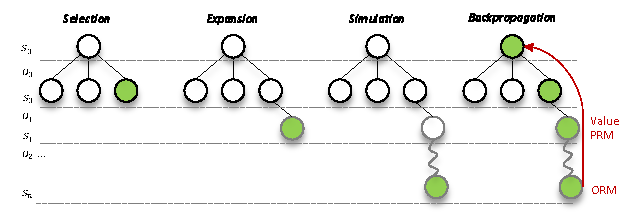
\includegraphics[width=\textwidth]{figures/emcts.pdf}
    \caption{An overview of the four operations of \emcts{}. A node is selected, expanded, simulated with fast rollout policy until a terminal node is reached, then the signals from value function, \prm{} and \orm{} are backpropagated.}
    \label{fig:emcts}
\end{figure}

\subsubsection{Option-level MCTS}

\begin{table}[!htb]
\footnotesize
    \centering
    \setlength{\tabcolsep}{4pt}
    \begin{tabular}{c|c|c}

    \toprule
    \texttt{Search Node} & \texttt{Example} & \texttt{Termination}  \cr
    \midrule
    Token-level & $y_0 \rightarrow y_1 \rightarrow y_2 \rightarrow y_3 \rightarrow y_5 \rightarrow y_6 \rightarrow y_7 \rightarrow y_8$ &  token\cr
    \midrule
    Sentence-level & $y_0 y_1 y_2$ \enterkey{}  $\rightarrow y_4 y_5 y_6$ \enterkey{} $\rightarrow y_7 y_8 y_9 y_{10}$ & new line\cr
    \midrule
    Option-level & $y_0$  $\rightarrow y_1 y_2$ \enterkey{} $\rightarrow y_4 y_5 y_6$ \enterkey{} $y_7 y_8 y_9$ \enterkey{} $\rightarrow y_{10}$& termination function\cr
    \bottomrule
    \end{tabular}
    \vspace{2mm}
    \caption{Comparative illustration of token-level, sentence-level, and option-level MCTS search nodes. $y$ denotes a token sampled from the policy model. The arrow $\rightarrow$ represents the transition from one search node to the subsequent node within the search process.}
    \label{tab:option}
\end{table}


% To apply MCTS to LLMs, it is naturally ~\cite{liu2023making} to performing search at the token-level, considering each token as an action. However, due to the typically large vocabulary size in LLMs, conducting a deep search becomes very challenging as the search space grows exponentially. Some attempts propose sentence-level search where each sentence or step is regarded as an action. While sentence-level search can reduce the complexity of the search space, it might affect the flexibility and performance applying MCTS to LLM as for some tasks subtle variations of several tokens could significantly alter the reward and some tasks might requires more than sentence level search, such as paragraph level search.

% However, the typically large vocabulary of LLMs poses a significant challenge, as conducting a deep search becomes increasingly difficult due to the exponential growth of the search space.

When applying MCTS to LLMs, it is natural to perform token-level search, where each token is considered as an action~\citep{liu2023making}. However, the substantial vocabulary size typical of LLMs presents a significant challenge \ie conducting a deep search in such a vast space becomes increasingly complex as the search space expands exponentially. To mitigate this, some efforts proposed a sentence-level search, treating each sentence or step as a search node~\citep{feng2023alphazero}. While this method reduces the search space, it might compromise the flexibility and effectiveness of applying MCTS to LLMs, which is particularly true for tasks where subtle variations in token can dramatically impact the outcome, or where a more comprehensive search beyond a sentence is necessary.

Inspired by~\cite{option_mcts, de2016monte}, we use the term option as a search node and propose option-level MCTS where each option represents a sequence of tokens, which can range from multiple tokens to several sentences. A comparisons of different levels search is listed in Table~\ref{tab:option}. Mathematically, an option $o = \langle \gI, \pi, \beta \rangle$, where $\gI \subseteq \gS$ is a set of initial states for the option; $\pi: \gS \times \gA \rightarrow [0,1]$ is a policy to generate actions, which in our case is a LLM; and $\beta: \gS^{+} \rightarrow [0,1]$ is the termination function. Starting from a state $s_t$, we can choose all the options for which $s_t \in \gI$. Once an option is chosen, the policy $\pi$ will generate actions for several steps until the option terminates according to the termination function $\beta$. The option-level MCTS consists of stages including selection, expansion, simulation, and backpropagation. The option-level formulation offers more flexibility compared to the sentence-level, as a new line can be treated as a special case of the termination function, as demonstrated in Table \ref{tab:option}. Additional detailed steps of the option-level MCTS can be found in Appendix \ref{app:option_level_mcts}.

% As illustrated in Figure~\ref{fig:emcts}, option-level MCTS consists of the following operations:
% \begin{itemize}[noitemsep,topsep=0pt,parsep=2pt,partopsep=0pt,leftmargin=*]
% \item \textbf{Selection} Starting from the root node, we iteratively select the child node based on Equation \ref{eqs:ucb}.
% \item \textbf{Expansion} Once an expandable leaf node is selected, a new node is generated by starting with the previous state of the parent node as the initial option state. The option is then sampled using the policy $\pi$, and its completion is determined by the termination function $\beta$. 
% \item \textbf{Simulation} The scaled reward of the newly expanded node, as well as some simulated future trajectories are evaluated using the feedback functions, which will be discussed in \S \ref{sec:critic}.
% \item \textbf{Backpropagation} The average value of the newly generated node and all its ancestors is updated using the scaled reward from the evaluation step. Meanwhile, the visit counts for these nodes are also increased by one.
% \end{itemize}

% \begin{itemize}[noitemsep,topsep=0pt,parsep=0pt,partopsep=0pt]
%   \item \paragraph{Selection} Starting from the root node, we iteratively select the child node based on Equation \ref{eqs:ucb}.
% \end{itemize}

%   \item \paragraph{Selection} Starting from the root node, we iteratively select the child node based on Equation \ref{eqs:ucb}.

% \item \paragraph{Expansion} Once an expandable leaf node is selected, a new node is generated by starting with the previous state of the parent node as the initial option state. The option is then sampled using the policy $\pi$, and its completion is determined by the termination function $\beta$. 
%   \item \paragraph{Simulation} The scaled reward of the newly expanded node, as well as some simulated future trajectories are evaluated using the feedback functions, which will be discussed in \S \ref{sec:critic}.
%   \item \paragraph{Backpropagation} The average value of the newly generated node and all its ancestors is updated using the scaled reward from the evaluation step. Meanwhile, the visit counts for these nodes are also increased by one.

% Employing an option to substitute a single token within each node could reduces search space, as the number of options in a trajectory is much smaller than the number of tokens. This facilitates a deeper search, broader coverage of the search space, and minimizes the frequency of requesting feedback from functions such as the value model. Moreover, the option-level offers more flexibility compared to the sentence-level, as a new line can be treated as a special case of the termination function, as demonstrated in Table \ref{tab:option}.

% Policy over options: $\mu: S \times O \rightarrow [0, 1]$ %

% --
% In previous works such as AlphaZero~\cite{silver2018general}, a search tree is built at every step, and the next action is selected based on certain root node statistics, such as visitation frequency. After performing the selected action and receiving the updated state from environment, the tree is built again. This approach is adopted due to the stochasticity of the environment, which requires building the tree based on the most recent actual move. However, in the case of text generation, as the state transition $T$ is deterministic, it is possible to build the tree only once, since all states are accurate. Starting from the initial state, the select-expand-evaluate-backup process is performed several times until a specified condition is met, such as the maximum number of rollouts or terminated nodes. The final answer is then selected from the tree by choosing the optimal trajectory. This offline version of MCTS has also been employed in~\cite{feng2023alphazero}.


% \subsubsection{Importance Weighted Expansion}
% % % Importance weighted expansion
% In previous work related to option/sentence level tree search ~\cite{feng2023alphazero, yao2024tree}, it has been a common practice to assume that each node in the tree has the same predefined width \ie branching factor. This is due to the fact that unlike token-level MCTS with a limited action space, the sample space at the option-level is exceedingly large, with an unlimited number of token combinations. Consequently, it is necessary to set a predefined maximum width and often result in an inefficient search space. For a given node, the error lead by the the branching factor limit can be formulated as
% \begin{equation*}
% E_{\phi} = \mathop{\mathbb{E}}[\min_{i}|v_{\phi}^{\pi}([\vs_t,\vo_t^{new}])-v_{\phi}^{\pi}([\vs_t,\vo_t^{i}])|]
% \end{equation*}
% where $\vo_t^{new}$ is the option of a potential new children that can not be added, $\vo_t^{i}$ represents the current ith children, and $v_{\phi}^{\pi}$ is the value function which will be detailed in \S \ref{sec:critic}. For now we assume that the value of the maximum $m_t$ children nodes are uniform distribution (which is not true but we will cover this in the next part). It is straightforward to show that 
% \begin{equation*}
% E_{\phi} \le \frac{\max_{\vo_t} |v^{\pi}([\vs_t,\vo_t])- v^{\pi}(\vs_t)|}{m_t}.
% \end{equation*}
% While the $E_{\phi}$ is less than some $\epsilon$, we want to use less total number of node for efficiency. And this thus can be formulate as an optimization problem:
% \begin{align*}
% \text{minimize:} & \sum m_t\\
% \text{subject to:} & \frac{\max_{i} |v^{\pi}([\vs_t,\vo_t^{i}])- v^{\pi}(\vs_t)|}{m_t} \le \epsilon
% \end{align*}
% We showed in Appendix that the optimal choice of $m_t$ is proportional to $\frac{1}{m_t}\max_{i} |v^{\pi}([\vs_t,\vo_t^{i}])- v^{\pi}(\vs_t)|$ constant of $1/(\epsilon)$. We name this part as importance $I(\vs_t)$, of the node $\vs_t$.
% \begin{equation*}
% % I(s_t) = \max_{a_t} |Q^{\pi}(s_t,a_t)- E_{a\sim\pi}[Q^{\pi}(s_t,a_t)]|
% I(\vs_t) = \max_{\vo_t} |v^{\pi}([\vs_t,\vo_t])- v^{\pi}(\vs_t)|
% \end{equation*}

% % A more effective and efficient way to determine the branching factor for each node is to dynamically adjust it based on the importance of each node. This approach allows us to allocate a larger child budget to nodes of higher importance, thereby preventing inefficient exploration of these nodes and ensuring that we do not miss promising solutions. Meanwhile, by reducing the number of children for less important nodes, we can perform deeper searches at various levels of the tree, rather than considering all possible options at each node. 

% Similar concept has also be proposed in ~\cite{taylor2014reinforcement, clouse1996integrating}. Intuitively, $I(\vs_t)$ captures the maximum value deviation from the current state. When this value is small, there is no need to explore further on this node, as there will not be a significant difference by rolling out on this node. Conversely, if the value is large, it is worth trying different children. We set the number of children allowed for a node $n(\vs_t)$ to be linear with this importance, using a factor $\alpha$. In practice, to avoid extreme cases of large variance of $I(\vs_t)$ in the early stage, we bound the number of children by depth-dependent constants $c_{\mathtt{min}}(t)$ and $c_{\mathtt{max}}(t)$:
% \begin{equation*}
% n(\vs_t) = \max\left(c_{\mathtt{min}}(t), \min\left(\lfloor \alpha I(\vs_t) \rfloor, c_{\mathtt{max}}(t)\right)\right).
% \end{equation*}

% \subsubsection{Efficient MCTS}
\subsubsection{Importance-Based Adaptive Branching}

In previous works related to option/sentence level tree search ~\citep{feng2023alphazero, yao2024tree}, it was a common practice to assume that each node in the tree has the same predefined width, \textit{i.e.}, branching factor. This assumption was due to the fact that unlike token-level MCTS with a limited action space, the sample space at the option-level is exceedingly large, with an unlimited number of token combinations. As a result, it was necessary to set a predefined maximum width for each node. However, this predefined branching factor is hard to set, as an improper choice can lead to a search tree that is either too shallow or too thin, resulting in an inefficient exploration of the search space.
% As a result, it was necessary to set a predefined maximum width,  which, however, often leads to an inefficient search space.

% \begin{equation*}
% E_{\phi}(t) = \mathop{\mathbb{E}_{\vo_t^{j}\sim \pi(\vs_t)}}[\min_{\vo_{t}^{i}}|v_{\phi}^{\pi}([\vs_t,\vo_t^{j}])-v_{\phi}^{\pi}([\vs_t,\vo_t^{i}])|]
% \end{equation*}
% \begin{equation*}
% I(\vs_t) = \max_{\vo_{t}^{i}} |v_{\phi}^{\pi}([\vs_t,\vo_t^{i}])- v_{\phi}^{\pi}(\vs_t)|
% \end{equation*}
To quantify the error induced by the branching factor limit, we defined the branching error \(E_{\phi}(t)\). For a node \(t\) with a branching factor of \(m_t\), it aims to use the \(m_t\) child options \(\vo_{t}^{i} \sim \gD_{t}^{children}\) (where \(i \in \{1, \ldots, m_t\}\)) to represent all possible options. Consequently, for a legal option \(\vo_{t}^{j} \sim \pi(\vs_t)\) from the option space, we can calculate the minimal value difference between it and the \(m_t\) existing options, which captures the error associated with representing other possible options using the \(m_t\) available options. It can be formulated as 
$E_{\phi}(t) = \mathop{\mathbb{E}_{\vo_t^{j}\sim \pi(\vs_t)}}[\min_{\vo_{t}^{i}}|v_{\phi}^{\pi}([\vs_t,\vo_t^{j}])-v_{\phi}^{\pi}([\vs_t,\vo_t^{i}])|]$, where $v_{\phi}^{\pi}$ is the value function which will be detailed in \S \ref{sec:critic}. Here we define the importance of node $\vs_t$ as $I(\vs_t) = \max_{\vo_{t}^{i}} |v_{\phi}^{\pi}([\vs_t,\vo_t^{i}])- v_{\phi}^{\pi}(\vs_t)|.$ For simplicity, we assume that the value of the children nodes are uniformly distributed (a detailed analysis of the Gaussian distribution can be found in Appendix \ref{app:node_importance_gaussian}). Under this assumption, we show in Appendix \ref{app:node_importance_uniform} that $E_{\phi}(t) \le \frac{I(\vs_t)}{m_t-1}.$
% \begin{equation*}
% E_{\phi}(t) = \frac{I(\vs_t)}{m_t-1}.
% \end{equation*}
While $E_{\phi}$ is less than some $\epsilon$, we aim to use a smaller total number of nodes for efficiency. 
% This can be formulated as an optimization problem:
% \begin{align*}
% \text{minimize:} & \sum m_t\\
% \text{subject to:} & \frac{I(\vs_t)}{m_t} \le \epsilon
% \end{align*}
\newtheorem{theorem}{Theorem}[section]
\begin{theorem}\label{thm:optimal_branching_factor}
The optimal branching factor $m_t$ in a tree search is set such that $m_t - 1$ is proportional to the node importance $I(\vs_t)$, under the condition $\frac{I(\vs_t)}{m_t-1} \le \epsilon$. \normalfont{Refer to Appendix \ref{app:node_importance_uniform} for the detailed proof.}
\end{theorem}
% \begin{proof}
% See Appendix \ref{app:node_importance_uniform}.
% \end{proof}

A similar concept has also been proposed in ~\cite{taylor2014reinforcement, clouse1996integrating}. Intuitively, $I(\vs_t)$ captures the maximum value deviation from the current state. When this value is small, there is no need to explore further on this node, as there will not be a significant difference by rolling out on this node. Conversely, if the value is large, it is worth trying different children. We set the number of children allowed for a node $n(\vs_t)$ (after extracting $1$) to be linear with this importance, using a factor $\alpha$. In practice, to avoid extreme cases of large variance of $I(\vs_t)$ in the early stage, we bound the number of children by depth-dependent constants $c_{\mathtt{min}}(t)$ and $c_{\mathtt{max}}(t)$, $n(\vs_t) = \max\left(c_{\mathtt{min}}(t), \min\left(\lfloor \alpha I(\vs_t) \rfloor+1, c_{\mathtt{max}}(t)\right)\right).$
% \begin{equation*}
% n(\vs_t) = \max\left(c_{\mathtt{min}}(t), \min\left(\lfloor \alpha I(\vs_t) \rfloor+1, c_{\mathtt{max}}(t)\right)\right).
% \end{equation*}

\subsubsection{State Merge}

% With $n(\vs_t)$ determined, another issue is that options under the same node are very similar, leading to many unnecessary sub-trees. Intuitively, we want the distribution of their values to be spread out. As shown in Appendix \ref{app:node_merge}, given a set of values that are evenly distributed, the worst-case error induced by the branching factor limit is minimized.

% Since we cannot directly control the $\vo_t \sim \pi(\vs_t)$, one strategy to make the value distribution of child nodes more evenly spread is to utilize the concept of move groups ~\cite{van2012revisiting}. By merging similar nodes into the same group, we can potentially influence the minimal value gaps between children. This merging allows us to increase the diversity among groups, thereby covering a larger problem space with limited search rollouts and making the search process more efficient.

% Here, we adapt the definition of node predicate $p_{vM}$ from ~\cite{abel2018state} and ~\cite{fu2024accelerating} to represent whether two nodes are extremely similar. In practice, each time we generate a new option from the policy, we use heuristic functions as $p_{vM}$ to check its similarity with all existing groups. The heuristic function can either be a faster rule-based measurement (e.g., edit distance) or a model-based method (e.g., prompting a language model). Based on this, we decide whether to merge this option with a previous one or create a new group. 

With $n(\vs_t)$ determined, another issue is that options under the same node may be very similar, leading to many unnecessary sub-trees. Since we cannot directly control the $\vo_t \sim \pi(\vs_t)$, one strategy to mitigate this issue is to utilize the concept of move groups, as discussed in ~\cite{van2012revisiting}. By merging similar nodes into the same group, we can increase the diversity among groups, thereby covering a larger problem space with limited search rollouts and making the search process more efficient.

Here, we adapt the definition of node predicate $p_{vM}$ from ~\cite{abel2018state} and ~\cite{fu2024accelerating} to represent whether two nodes are extremely similar. In practice, each time we generate a new option from the policy, we use heuristic functions as $p_{vM}$ to check its similarity with all existing groups. The heuristic function can either be a faster rule-based measurement (e.g., edit distance) or a model-based method (e.g., prompting a language model). Based on this, we decide whether to merge this option with a previous one or create a new group. 

% Another explanation, as shown in Appendix \ref{app:node_merge}, is that given a set of values that are evenly distributed, the worst-case error induced by the branching factor limit is minimized. Intuitively, the state merge can also help make the value distribution of child nodes more evenly spread (although not absolutely, as different states may also have similar values).

\subsubsection{Fast Rollout with Specialized LM}

The simulation operation which employs a rollout policy to project future trajectories from a given state, is crucial for an effective MCTS. This process significantly improves the efficiency of exploration and exploitation, and enhances the accuracy of reward estimation\footnote{Typically, the closer the simulation is to the termination state, the more accurate the reward estimation becomes.}. Estimations made at the end of trajectories tend to have lower bias but higher variance; thus, simulating multiple possible trajectories yields low-bias, low-variance estimates, enabling a more informed and effective search process. Ideally, $\pi_\theta$ would serve as the rollout policy, yet its computational demands render it impractical for the rapid simulations required by MCTS. To address this challenge, we propose the use of a smaller, specialized LM as the fast rollout policy $\pi^{\mathtt{fast}}$. Given a state $\vs_t$, the fast rollout policy $\pi^{\mathtt{fast}}$ efficiently continues generation until it reaches a termination condition, denoted as $\pi^{\mathtt{fast}}(\vs_t)$.

\subsection{Critic}
\label{sec:critic}
% It is crucial for searching algorithms to have reliable guidance signals towards achieving the end goal. 
% In \model{}, we design three types of critic models to guide the search process, \ie value function $v^\pi$ predicting the future reward, process reward models \texttt{PRM} estimating node quality, and outcome reward model \texttt{ORM} assessing the overall trajectory quality. 

In \model{}, we design three types of critic models to guide the search process.

% \paragraph{Value Function} The value function, denoted as $v^\pi(\vs)$, is the expected return starting from state $\vs_t$ following the policy $\pi$ thereafter. To train a value function $v^\pi_\phi(\vs)$ parameterized by $\phi$ ~\citep{feng2023alphazero}, we use the Monte Carlo (MC) estimate to empirically approximate the expected reward by averaging the rewards observed after many samplings starting from state $s$ and following policy $\pi$. Thus, the MC estimate of $v^\pi_\phi(\vs)$ can be written as $v^\pi_\phi(\vs) \approx \frac{1}{J} \sum_{j=1}^{J} G^{(j)}(\vs)$ where $J$ is the number of trajectory starting from state $\vs$, $G^{(j)}(\vs)$ is the total discounted reward from state $s$ in the $j$-th trajectory. Particularly, given the expert demonstration dataset $\gD = \{(\vx_i, \vy_i)\}$, for each prompt $\vx_i$, we generate trajectories $\vtau_i^j = \{\vx_i, \vo_{i1}^j, \vo_{i2}^j, \cdots, \vo_{iT}^j \}$ by following policy $\pi$. A reward $r_i^j$ is assigned to indicate whether $\vtau_i^j$ aligns with $\vy_i$, \eg rewarding trajectories that contains correct answers in mathematical tasks or closely follows the instruction as the ground-truth. We then construct a dataset $\gD_{\mathtt{value}} = \{ (\vs_{it}, v_{it}) | i\in[N], t\in[T]\}$ in which $\vs_{it} = [\vx_i\cdot\vo_{<it}]$ and $v_{it} = \frac{1}{J} \sum_{j=1}^{J} r^j_{iT}$. The value function $v_\phi^\pi$ is optimized by minimizing mean squared error $\gL_\phi = - \sE_{(\vs, v)\sim \gD_{\mathtt{value}}} (v_\phi^\pi(\vs) - v)^2$.
% % \begin{equation*}
% % \gL_\phi = - \sE_{(\vs, v)\sim \gD_{\mathtt{value}}} (v_\phi^\pi(\vs) - v)^2
% % \end{equation*}
% We opt to initialize $v_\phi^\pi$ using the parameters from policy $\pi_\theta$, incorporating an MLP layer on top of it to output a scalar on each token. The scalar prediction at the last token of each state is used as the value.
% %, which can be further written as $G_t^{(i)}(s) = \sum_{k=0}^{\infty} \gamma^k R_{t+k+1}^{(i)}$ in which $R_{t+k+1}^{(i)}$ represents the reward received at time $t+k+1$ in the $i$-th trajectory, and $\gamma$ is the discount factor, with $0 \leq \gamma \leq 1$. We create the 

\paragraph{Value Function} The value function, denoted as $v^\pi(\vs)$, represents the expected return starting from state $\vs$ and following policy $\pi$ thereafter, given by $v^\pi(\vs) = \mathop{\mathbb{E}}_{\tau \sim \pi}[R(\tau)|s_0 = \vs]$ where $R(\tau)$ represents the discounted return of trajectory $\tau$. To train a parameterized value function $v^\pi_\phi(\vs)$, given the prompts $\gD = \{(\vx_i, \cdots) \mid i \in [N]\}$, for each prompt $\vx_i$, we generate multiple trajectories $\vtau_i^j = \{\vx_i, \vo_{i1}^j, \vo_{i2}^j, \cdots, \vo_{iT}^j \}$ by following policy $\pi$ for $J$ times. A final reward $r_i^j$ is assigned to indicate whether $\vtau_i^j$ aligns with $\vy_i$—for example, rewarding trajectories that contain correct answers in mathematical tasks or closely follow instructions as ground truth. We then construct a dataset $\gD_{\mathtt{value}} = \{ (\vs^j_{it}, v^j_{it}) \mid i \in [N], t \in [T], j \in [J] \}$ where $\vs^j_{it} = [\vx_i \cdot \vo^j_{<it}]$ and $v^j_{it} = r^j_i$. The value function $v_\phi^\pi$ is optimized by minimizing the mean squared error: $\gL_\phi = - \sE_{(\vs, v) \sim \gD_{\mathtt{value}}} (v_\phi^\pi(\vs) - v)^2$. Similar to ~\citep{feng2023alphazero}, $v_\phi^\pi$ is a LLM with an MLP layer on top to output a scalar on each token, using the scalar prediction at the last token of each state as the value.

% \begin{equation*}
% \gL_\phi = - \sE_{(\vs, v) \sim \gD_{\mathtt{value}}} (v_\phi^\pi(\vs) - v)^2
% \end{equation*}

\paragraph{PRM} The value function often struggles with credit assignment problem~\citep{sutton1984temporal} and its learning could be inefficient due to delayed and sparse rewards~\citep{sutton2018reinforcement}. Therefore, we propose to incorporate \prm{} that introduces process supervision~\citep{lightman2023let} for direct option assessment. \prm{} generates intrinsic rewards~\citep{chentanez2004intrinsically} to encourage explorations of advantageous options, effectively mitigating issues of reward sparsity by providing immediate, action-specific rewards. Given a state $\vs_t$ and an option $\vo_t$ at time $t$, the \prm{} aims to predict the immediate reward $r_t^{\texttt{PRM}}$ that results from taking option $\vo_t$ in state $\vs_t$. Formally, the \prm{} is a function $R(\vs_t, \vo_t) \rightarrow r^{\mathtt{PRM}}_t$. While \prm{} ideally requires quality labels for each state ~\citep{uesato2022solving}, due to the high cost and time involved in obtaining these, MC estimation with prefix sampling~\citep{wang2023math} is used as a proxy, which aligns with the objective of the value function. Instead of adding a MLP layer on top of the policy model for outputting a scalar reward~\citep{ouyang2022training}, we formulate \prm{} as a text generation task to best leverage LLM's intrinsic knowledge for assessing the quality of an option. We adapt the dataset constructed for the value function as $\gD_{\mathtt{PRM}} = \{ (\vs_{it}, \vo_t, r_t^{\mathtt{PRM}} ) | i\in[N], t\in[T]\}$ where $r_t^{\mathtt{PRM}}$ is the textual description of the reward, \eg an option can be regarded as good if $v_{it}$ is larger than certain threshold. To train \prm{},  we initialize it from the policy model $\pi$ and use the following prompt templates and typical language model loss. The prompt template is shown in Appendix \ref{app:prompt}.

% \begin{tcolorbox}[label=prm_prompt]
% \#\#\#[A detailed rubric that specifies how to evaluate a step of a task]\textbackslash n\textbackslash n\#\#\# State\textbackslash n\{\texttt{state}\}\textbackslash n\textbackslash n\#\#\#Action\textbackslash n\{\texttt{option}\}\textbackslash n\textbackslash n\#\#\#Assessment\textbackslash n\{\texttt{textual reward}\}
% \end{tcolorbox}

\paragraph{ORM} In additional to the value function and \prm{}, \orm{} is also used to guide MCTS. \orm{} is designed to evaluate options sequences in their entirety, assessing the extent to which the complete trajectory aligns with the desired end goal~\citep{uesato2022solving,lightman2023let,wang2023math,feng2023alphazero}. The outcome evaluation complements value function and \prm{} by offering a comprehensive assessment of trajectories. Crucially, \orm{} plays a vital role in the simulation stage of MCTS by providing more accurate signals on the terminal state, which in turn facilitates a more balance between exploration and exploitation strategies. \orm{} is formulated as a text generation task, similar to \prm{}. We leverage the same dataset for the value function training and construct $\gD_{\mathtt{ORM}} = \{ (\vx_i, \vo_{1:T}^i, r_i^{\mathtt{ORM}}) | i\in[N]\}$, where each instance includes a initial state or prompt $\vx_i$, a sequence of actions or options $\vo_{1:T}^i$ taken from that state, and a textual reward $r_i^{\mathtt{ORM}}$ indicating the sequence's success or quality. Similarly, \orm{} is initialized from the policy model $\pi$ and the following prompt templates and language model loss are used for training. The prompt template is shown in Appendix \ref{app:prompt}. \\
% \begin{tcolorbox}
% \#\#\#[A detailed rubric that specifies how to evaluate a complete trajectory of a task]\textbackslash n\textbackslash n\#\#\# Prompt\textbackslash n\{\texttt{prompt}\}\textbackslash n\textbackslash n\#\#\#Trajectory\textbackslash n\{\texttt{trajectory}\}\textbackslash n\textbackslash n\#\#\#Assessment\textbackslash n\{\texttt{textual reward}\}
% \end{tcolorbox}

% provide precision feedback on exploirtation

% \begin{equation*}
% s(\vs) = \beta_{\text{value}} \cdot v_\phi^\pi(\vs) + \beta_{\text{PRM}} \cdot \prm{}(\vs) + \beta_{\text{ORM}} \cdot \mathbb{E}_{\tau \sim \pi^{\mathtt{fast}}(\vs)} [\orm{}(\tau)]
% \end{equation*}

The final score evaluation of a state $\vs$ is a weighted sum of the value function, \prm{}, and \orm{}: $s(\vs) = \beta_{\text{value}} \cdot v_\phi^\pi(\vs) + \beta_{\text{PRM}} \cdot \prm{}(\vs) + \beta_{\text{ORM}} \cdot \mathbb{E}_{\tau \sim \pi^{\mathtt{fast}}(\vs)} [\orm{}(\tau)]$, where $\tau \sim \pi^{\mathtt{fast}}(\vs)$ represents trajectories starting from $\vs$ under $\pi^{\mathtt{fast}}$, and $\beta_{\text{value}}$, $\beta_{\text{PRM}}$, $\beta_{\text{ORM}}$ are hyperparameters. In practice, we found that the value function model has better precision and calibration, while \prm{} has superior recall (Appendix \ref{app:critic_performance}). Although \orm{} with fast rollouts provides low-bias, low-variance estimates, it still inherits some bias from $\pi^{\mathtt{fast}}$. Thus, combining these critics yields a stronger evaluation signal.

\subsection{Policy Self-Improvement}
\label{sec:self_improve}

% We have discussed how \emcts{} can guide policy to find trajectories of higher quality and. In this subsection, we discuss how to leverage these trajectories to further improve the policy. It is an iterative process with each iteration containing two main steps: \emph{data generation} and \emph{policy finetuning}.
The policy improvement an iterative process with each iteration containing two main steps: \emph{data generation} and \emph{policy finetuning}.
\paragraph{Data generation} In this step, we assume to have the current policy $\pi_{\theta_k}$ and synthetic prompts $\gD_k=\{\vx^k_1,\dots\}$ at the $k$-th round, where each $\vx^k_1$ represents a question.
We obtain the corresponding training data $\gD_k$ for policy $\pi_{\theta_k}$ by firstly performing \emcts{} on $\gD_k$ (\S \ref{sec:mcts}) and then sampling a trajectory $\vy^k_i$ from the corresponding tree for each question $\vx^k_i$.
% There are several ways to select a trajectory from a MCTS forest, such as taking a greedy path based on the critic score ($w_i$ in Eq. \ref{eqs:ucb}).
Here we choose the trajectory that yield the highest critic score on the leaf node for each input question.
Next, we filter out instances where the corresponding trajectory is substandard forming $\gD_k = \{(\vx^k_i, \vy^k_i)~|~f(\vx^k_i, \vy^k_i)>\gamma\}$
% \begin{equation*}
%  \gD_k = \{(\vx^k_i, \vy^k_i)~|~f(\vx^k_i, \vy^k_i)>\gamma\}
% \end{equation*}
where $f$ represents a function for quality scoring, and $\gamma$ indicates a threshold.
There can be several ways to implement the function, and here we simply use the \orm{} (\S \ref{sec:critic}).

% In this step, we assume to have the current policy $\pi_{\theta_k}$, value network $v^{\pi}$, \orm{} and synthetic prompts $\gD=\{\vx^k_1,\dots\}$, where each $\vx^k_1$ represents a question.
% We obtain the corresponding training data $\gD_k$ for policy $\pi_{\theta_k}$ by first performing MCTS on $D$ (\S \ref{sec:mcts}) and then sampling a trajectory $\vy^k_i$ from the corresponding MCTS forest for each question $\vx^k_i$.
% There are several ways to select a trajectory from a MCTS forest, such as taking a greedy path based on the critic score ($w_i$ in Eq. \ref{eq:mcts}).
% Here we choose the trajectory that yield the highest critic score on the leaf node for each input question.
% As the next step, we filter out instances where the corresponding trajectory is not in high quality:


% consider whether the the final answer of $y^i$ correct (equals to $a^i$).

\paragraph{Policy finetuning}
% With the obtained training data $\gD_k$, we organize the data into the following prompt templates $P_{SI}$:
With the obtained training data $\gD_k$, we organize the data into the prompt templates shown in Appendix \ref{app:prompt}. Then the policy $\pi_{\theta_k}$ is finetuned using target-loss: $\mathcal{L}_{\theta_k} = \mathbb{E}_{(\vx^k_i, \vy^k_i) \sim \gD_k} \big[\log \pi_{\theta_k}(\vy^k_i|\vx^k_i) \big]$, resulting in an updated policy $\pi_{\theta_{k+1}}$. We leave other training methods, such as DPO \citep{rafailov2023direct} or PPO \citep{schulman2017proximal} in future work.
% \begin{equation*}
%  \mathcal{L}_{\theta_k} = \mathbb{E}_{(\vx^k_i, \vy^k_i) \sim \gD_k} \big[\log \pi_{\theta_k}(\vy^k_i|\vx^k_i) \big]
% \end{equation*}
% This results in an updated policy $\pi_{\theta_{k+1}}$.
% We leave other training methods, such as DPO \citep{rafailov2023direct} or PPO \citep{schulman2017proximal} in future work.
% With the new policy, the value network and ORM is then updated as described in \S \ref{}.

% \section{Experiments}
% \label{sec:exp}
% 

% \subsection{Evaluation Setups}

\subsection{Experiment Setups}

\model{} is generally applicable to a wide spectrum tasks. As an early exploration, in this paper, we conduct experiments on mathematical reasoning problems where the learning signals are clear to define \ie, final answer is correct or wrong. We choose to evaluate on two widely used datasets GSM8K~\citep{gsm8k} and MATH~\citep{math}. For GSM8K, we utilize the whole test set while for MATH, due to computation constraints, we utilize a subset following the same procedure of~\cite{lightman2023let}. We evaluate the performance of predicting answers correctly for policy models. In addition, we calculate the average rollouts, represented by the number of nodes in the tree, as a measure of computational efficiency. We compare the performance of \model{} with a suite of proprietary model, including OpenAI's GPT-4 and GPT-3.5, Anthropic's Claude-2, as well as Google's PaLM-2 and the gemini model family. To ensure a fair and consistent evaluation, we employ CoT as our primary prompting method. Additionally, we conduct comparisons with strong open-source models, including Llama-2-70b~\citep{llama2} and WizardMath-70B-V1.0~\citep{wizardmath}. % For LLaMA-2 70B, we present results from few-shot prompting as well as zero-shot prompting for its SFT version, which was trained using CoT rationales and final answers. Wizardmath 70B has been trained on a diverse set of mathematical data generated by ChatGPT, employing both SFT and RLHF. We provide zero-shot prompting results.

%Means square errors and next token prediction accuracy are reported for evaluating value functions and \prm{}/\orm{}, respectively.
% \paragraph{Baseline Systems} We evaluate the performance of \model{} against a suite of proprietary model, including OpenAI's GPT-4 and GPT-3.5, Anthropic's Claude-2, as well as Google's PaLM-2 and the gemini model family. To ensure a fair and consistent evaluation, we employ CoT as our primary prompting method. We additionally report PAL~\citep{gao2023pal} prompting performance with GPT-4 as it demonstrates enhanced performance. Additionally, we conduct comparisons with strong open-source models, including LLaMA-2 70B~\citep{llama2} and Wizardmath 70B~\citep{wizardmath}. For LLaMA-2 70B, we present results from few-shot prompting as well as zero-shot prompting for its SFT version, which was trained using CoT rationales and final answers. Wizardmath 70B has been trained on a diverse set of mathematical data generated by ChatGPT, employing both SFT and RLHF. We provide zero-shot prompting results.

% The implementation details can be found in Appendix \ref{app:implementation}.


% \paragraph{Datasets} \model{} is generally applicable to a wide spectrum tasks. As an early exploration, in this paper, we conduct experiments on mathematical reasoning problems where the learning signals are clear to define \ie, final answer is correct or wrong. We choose to evaluate on two widely used datasets GSM8K~\citep{gsm8k} and MATH~\citep{math}. For GSM8K, we utilize the whole test set while for MATH, due to computation constraints, we utilize a subset following the same procedure of~\cite{lightman2023let}.
% \paragraph{Metrics} We evaluate the performance of predicting answers correctly for policy models. In the same time, we calculate the average rollouts, represented by the number of nodes in the tree, as a measure of computational efficiency. %Means square errors and next token prediction accuracy are reported for evaluating value functions and \prm{}/\orm{}, respectively.
% \paragraph{Baseline Systems} We evaluate the performance of \model{} against a suite of proprietary model, including OpenAI's GPT-4 and GPT-3.5, Anthropic's Claude-2, as well as Google's PaLM-2 and the gemini model family. To ensure a fair and consistent evaluation, we employ CoT as our primary prompting method. We additionally report PAL~\citep{gao2023pal} prompting performance with GPT-4 as it demonstrates enhanced performance. Additionally, we conduct comparisons with strong open-source models, including LLaMA-2 70B~\citep{llama2} and Wizardmath 70B~\citep{wizardmath}. For LLaMA-2 70B, we present results from few-shot prompting as well as zero-shot prompting for its SFT version, which was trained using CoT rationales and final answers. Wizardmath 70B has been trained on a diverse set of mathematical data generated by ChatGPT, employing both SFT and RLHF. We provide zero-shot prompting results.

% The implementation details can be found in Appendix \ref{app:implementation}.
% \subsection{Baseline Systems}
% We evaluate the performance of \model{} against a suite of proprietary model, including OpenAI's GPT-4 and GPT-3.5, Anthropic's Claude-2, as well as Google's PaLM-2 and the gemini model family. To ensure a fair and consistent evaluation, we employ CoT as our primary prompting method. We additionally report PAL~\citep{gao2023pal} prompting performance with GPT-4 as it demonstrates enhanced performance.

% Additionally, we conduct comparisons with strong open-source models, including LLaMA-2 70B~\citep{llama2} and Wizardmath 70B~\citep{wizardmath}. For LLaMA-2 70B, we present results from few-shot prompting as well as zero-shot prompting for its SFT version, which was trained using CoT rationales and final answers. Wizardmath 70B has been trained on a diverse set of mathematical data generated by ChatGPT, employing both SFT and RLHF. We provide zero-shot prompting results.

% We conduct our experiments on two math datasets, GSM8K~\citep{gsm8k} and MATH~\citep{math}.
% Our use LLaMa 2 70B~\citep{llama2} and WizardMath 70B V1.0~\citep{wizardmath} as our base models for GSM8K and MATH respectively.

% \subsection{Implementation Details}

We select Llama-2-70b as the policy model for the GSM8K dataset and WizardMath-70B-V1.0 for the MATH dataset. To construct the training dataset for the value function, \prm{} and \orm{}, we generate 50 trajectories for each prompt and construct the training target following Section~\ref{sec:critic}. Both \prm{} and \orm{} are initialized using the weights from the policy model, while the value function uses a smaller Llama-2-13b model, as we observed no performance gains from increasing the value function model size. In the design of \orm{}, tool usage is not incorporated for GSM8K. However, for MATH, we enhance \orm{} by incorporating tools like python sympy to assess the quality of a trajectory, in a manner similar to that described by \citet{gou2023tora}. The training employ a learning rate of 1e-6 and are trained for one epoch. For the fast rollout policy model, we opt for the Abel-002-7B model~\citep{abel} for both the GSM8K and MATH tasks for its high efficiency and superior performance. For the MCTS parameters, they are configured at different scales, as shown in Appendix \ref{app:implementation}. We set $\beta_{\text{value}}$, $\beta_{\text{PRM}}$, and $\beta_{\text{ORM}}$ all to 1.0.

% We set the MCTS parameters as follows: in GSM8K, $c=1$ for the small scale (\texttt{\#rollout}) and $1.5$ for the large scale, with $\alpha=1$. For $t=0$, $c_\text{min}(0)=10$ for the small scale and $40$ for the large scale, while for the rest of $t$, $c_\text{min}(t)=2$. We also set $c_\text{max}(0) = 10$ for the small scale and $40$ for the large scale, and for the remaining $t$, $c_\text{max}(t)=10$. The termination condition is based on sentence termination. In MATH, the parameters are $c=1$, $\alpha=1$, and for $t=0$, $c_\text{min}(0)=10$ for the small scale and $20$ for the large scale, while for the rest of $t$, $c_\text{min}(t)=3$. We set $c_\text{max}(0) = 10$ for the small scale and $20$ for the large scale, and for the remaining $t$, $c_\text{max}(t)=10$. The termination function is rule-based, checking if there are any formulations or calculations in the sentence. If there are, the option is terminated; otherwise, the option continues to extend.

For policy self-improving (\S \ref{sec:self_improve}), we train the policy model up to 3 epochs, setting batch size to 128, learning rate to $5\times 10^{-6}$ and minimal learning rate to $1\times 10^{-6}$.
Linear warm-up and decay is used with warm-up percent to be 10\%.
We perform early stopping based on a devset held out from the training instances.
For GSM8K experiments, we perform two rounds of self-improving, synthesizing 6.4k and 7.9k prompts\citep{yu2023metamath} respectively to obtain the corresponding MCTS outputs for training.
For MATH experiments, we only perform one round of self-improving due to limited computation resources, and 5.9k prompts are synthesized.

The termination function for options can be either be learned or rule-based. In practice, for the GSM8K dataset, the termination condition occurs at the end of each line. This is based on the typical structure of this dataset, where each line represents a distinct step or point. For the MATH dataset, due to its complexity and the base model's tendency to generate many \texttt{\textbackslash n\textbackslash n} line breaks with some less meaningful content between them, termination occurs at the end of a line if a formula pattern is detected. During inference, if \texttt{\textbackslash n\textbackslash n} is encountered, we perform a rule-based check for formula patterns. It terminates if a pattern is found or continues generating until the next \texttt{\textbackslash n\textbackslash n}.


\subsection{Results}
% Compare all existing approaches, add MATH results
% \begin{table}[!htb]
%     \centering
%     \begin{tabular}{ll|c|c}
%         \multicolumn{2}{l|}{Method}         & GSM8K  & MATH   \\
%         \hline
%         \multicolumn{2}{l|}{GPT-4 }         & $92.0$ & $42.5$ \\
%         \multicolumn{2}{l|}{GPT-4 (PAL)}    & $94.2$ & $51.8$ \\
%         \hline
%          \multirow{3}{*}{Gemini} & 1.0 Pro  & $77.9$ & $32.6$ \\
%          & 1.0 Ultra                        & $88.9$ & $53.2$ \\
%          & 1.5 Pro                          & $92.5$ & $58.5$ \\
%         \hline
%         \multicolumn{2}{l|}{ChatGPT}        & $80.8$ & $35.5$ \\
%         \multicolumn{2}{l|}{Claude-2}       & $85.2$ & $32.5$ \\
%         \multicolumn{2}{l|}{PaLM-2}         & $80.7$ & $34.3$ \\
%         \hline
%         \multicolumn{2}{l|}{LLaMA-2 70B}     & $57.8$ & $14.4$ \\
%         \multicolumn{2}{l|}{LLaMA-2 70B SFT} & $69.3$ & $14.9$ \\
%       % \multicolumn{2}{l|}{ToRA}            & $84.3$ & $49.7$ \\
%     \multicolumn{2}{l|}{WizardMath 70B V1.0} & $81.6$ & $22.7$ \\
%         \hline \hline
%         \multirow{2}{*}{MCTS} & Base model  & $88.9$ & $48.7$ \\
%          & Improved policy                  & $92.4$ & $51.0$   \\
%         \hline
%     \end{tabular}
%     \vspace{4mm}
%     \caption{Overall results on GSM8K and MATH test sets. 
%     We use LLaMA-2 70B and WizardMath 70B V1.0 as our base models on GSM8K and MATH data sets respectively. 
%     }
%     \label{tab:final_result}
% \end{table}

{
\renewcommand{\arraystretch}{1.05}
% \begin{table*}[!t]
% \centering
% \scalebox{1.1}{    
% 	\setlength\tabcolsep{6pt}
% 	% \begin{threeparttable}
% 		% \fontsize{9}{9}
% 		% \selectfont
% 		\begin{tabular}{lcc|cc}
% 			\toprule
% 			Model         & \texttt{IDD} & \texttt{SYN} & \texttt{GSM8K} & \texttt{MATH} \cr 
% 			\midrule
%     GPT-3.5~\cite{} & - & - & 80.8 & 35.5 \cr
%    GPT-4~\cite{} & - & - & 92.0 & 42.5 \cr
%    GPT-4 (PAL)~\cite{} & - & - & 94.2 & 51.8 \cr
%    \midrule
%    Gemini 1.0 Pro~\cite{} & - & - & 77.9 & 32.6 \cr
%    Gemini 1.0 Ultra~\cite{} & - & - & 88.9 & 53.2 \cr
%    Gemini 1.5 Pro~\cite{} & - & - & 92.5 & 58.5 \cr
%    \midrule
%    Claude-2~\cite{} & - & - & 85.2 & 32.5 \cr
%    PaLM-2 540B~\cite{} & - & - & 80.7 & 34.3 \cr
%    \midrule
%    LLaMA-2 70B & $\times$ & $\times$ & 57.8 & 14.4 \cr
%    LLaMA-2 70B SFT & $\checkmark$ & $\times$ & 69.3 & 14.9 \cr
%    WizardMath 70B V1.0 & $\times$ & $\times$ & 81.6 & 22.7 \cr
%    \midrule
%    \model{} & $\checkmark$ & $\times$ & 88.9 & 48.7 \cr
%    \model{} & $\checkmark$ & $\checkmark$ & 92.4 & 51.0 \cr
% 			\bottomrule  
% 		\end{tabular}
% 	% \end{threeparttable}
% 		  }
% 	\caption{Overall results on GSM8K and MATH test sets. 
%     We use LLaMA-2 70B and WizardMath 70B V1.0 as our base models on GSM8K and MATH data sets respectively. \texttt{IDD} indicates that the model has been trained using in-domain data. \texttt{SYN} denotes that the model has been trained on synthetic prompts, with trajectories generated using MCTS. }
% 	\label{table:main_results}
% \end{table*}

\begin{table*}[!t]
\small
    \centering
    % \scalebox{1.1}{    
        \setlength\tabcolsep{6pt}
        % \begin{threeparttable}
        % \fontsize{9}{9}
        % \selectfont
        \begin{tabular}{lccccc|cc}
            \toprule
            Model                    & \texttt{Decoding} & \texttt{\#Annotation} & \texttt{RN} & \texttt{FA} & \texttt{SYN} & \texttt{GSM8K} & \texttt{MATH} \cr 
            \midrule
            GPT-3.5~\cite{}          & Sampling & - & - & -             & -            & 80.8           & 35.5 \cr          
            GPT-4~\cite{}            & Sampling & -  & - & -          & -            & 92.0           & 42.5 \cr          
            GPT-4 (PAL)~\cite{}      & Sampling & -   & - & -         & -            & 94.2           & 51.8 \cr          
            \midrule
            Gemini 1.0 Pro~\cite{}   & Sampling & -   & - & -          & -            & 77.9           & 32.6 \cr          
            Gemini 1.0 Ultra~\cite{} & Sampling & -    & - & -         & -            & 88.9           & 53.2 \cr          
            Gemini 1.5 Pro~\cite{}   & Sampling & -     & - & -        & -            & 92.5           & 58.5 \cr          
            \midrule
            Claude-2~\cite{}         & Sampling & -     & - & -        & -            & 85.2           & 32.5 \cr          
            PaLM-2 540B~\cite{}      & Sampling & -      & - & -       & -            & 80.7           & 34.3 \cr          
            \midrule
            Llama-2-70b              & Greedy & 0 & $\times$ & $\times$ & $\times$         & 57.8           & - \cr          
            Llama-2-70b SFT          & Greedy & 7.5k & $\checkmark$ & $\checkmark$ & $\times$     & 69.3           & - \cr          
            WizardMath-70B-V1.0      & Greedy & 96k & $\checkmark$ & $\checkmark$ & $\times$         & -           & 20.7 \cr          
            \model{}                 & Greedy & 7.5k/7.5k & $\times$ & $\checkmark$ & $\checkmark$ & 73.7           & 23.6 \cr         
            \midrule
            \model{}                 & \emcts{} & 7.5k/7.5k & $\times$ & $\checkmark$ & $\times$      & 88.9           & 48.7 \cr          
            \model{}                 & \emcts{} & 7.5k/7.5k & $\times$ & $\checkmark$ & $\checkmark$  & 92.0           & 51.0 \cr                       
            \bottomrule   
        \end{tabular}
        % \end{threeparttable}
    
    % \caption{Comparison results of \model{} on the GSM8K and MATH datasets, utilizing LLaMA-2 70B and WizardMath 70B V1.0 as base models for GSM8K and MATH datasets, respectively. \texttt{\#Annotation} indicates the quantity of labeled data employed for fine-tuning each base model. The annotation used for training are noted as \texttt{RN} for rationales and \texttt{FA} for final answers. \texttt{SYN} means models trained on synthetic prompts, where trajectories were generated using \emcts{}. }

\caption{Comparison results of \model{} on the GSM8K and MATH datasets. \texttt{\#Annotation} indicates the quantity of labeled data employed for fine-tuning policy or training critic models. The annotation used for training are noted as \texttt{RN} for rationales and \texttt{FA} for final answers. \texttt{SYN} means models trained on synthetic prompts, where trajectories were generated using \emcts{}. }
    
    \label{table:main_results}
\end{table*}
}
% Table~\ref{table:main_results} presents the experimental results of \model{} on GSM8K and MATH. We observe that

Table~\ref{table:main_results} lists the performance comparisons of various methods on the GSM8K and MATH datasets. Our findings reveal that \model{}, based on Llama-2-70B and WizardMath-70B-V1.0, utilizes only final answer annotations and continues to improve through training on responses from \emcts{}. This comparison underscores the efficacy and broad applicability of our imagination-searching-criticizing self-improving framework. Moreover, when our model is augmented with \emcts{} decoding strategy, its performance markedly improves, achieving scores of 88.9 and 48.7 on the GSM8K and MATH datasets, respectively. Following two iterations of self-improvement using synthetic prompts, \model{} demonstrates performance comparable to that of GPT-4. This suggests a viable approach to improving LLMs' capabilities in complex problem-solving tasks in a self-improving fashion, leveraging a minimal amount of labeled data. We also analyze the performance of various search methods in Appendix \ref{app:search_comparison}.

% In addition, table~\ref{table:search_comparison} presents the performance of various methods applied to different number of responses, from 10 to 50. Our analysis confirms several key findings: 1) Reranking utilizing \orm{} consistently outperforms self-consistency techniques, indicating that \orm{} is capable of generating meaningful signals for searching. 2) \emcts{} demonstrates superior performance while requiring significantly fewer rollouts. For instance, on the MATH dataset, \emcts{} achieves better results with only half the number of rollouts compared to reranking. These results suggest that our design of an efficient MCTS in \model{} can serve as an effective policy improvement operation, enabling the search for high-quality trajectories with reduced computational cost.


\subsection{Ablation Study}
% % baseline (sampling)
% self consistence w/ diff. size of n-samples
% reranking w/ diff. size of n-samples
% MCTS w/ diff. size of rollout
% \begin{table}[!htb]
%     \centering
%     \setlength{\tabcolsep}{4pt}
%     \begin{tabular}{c||c|c|c||c|c|c}
%         \multirow{2}{*}{Method}           & \multicolumn{3}{c||}{GSM8K} &   \multicolumn{3}{c}{MATH} \\
%         \cline{2-7}
%             & \# of outputs & \# of rollouts  & Accuracy & \# of outputs & \# of rollouts  & Accuracy \\
%         \hline \hline
%         Baseline                          & $1$  & $4.6$ & $57.8$ & $1$ & $9.9$ & $20.7$ \\
%         \hline\hline
%         \multirow{3}{*}{Self-consistence} & $10$ & $46$  & $67.4$ &  $10$   &  $99$   & $22.5$ \\
%                                           & $30$ & $137$ & $74.2$ &  $30$   &  $299$  & $27.3$ \\
%                                           & $50$ & $229$ & $75.4$ &  $50$   &  $499$  & $28.8$ \\
%         \hline\hline
%         % MATH ORM V4 results: tool use
%         \multirow{3}{*}{Re-ranking}       & $10$ & $46$  & $80.8$ &  $10$   &  $99$   &  $34.1$ \\
%                                           & $30$ & $137$ & $86.3$ &  $30$   &  $299$  &  $39.0$ \\
%                                           & $50$ & $229$ & $87.7$ &  $50$   &  $499$  &  $42.0$ \\
%         % MATH ORM V2 results: no tool use for ORM
%         % \multirow{3}{*}{Re-ranking}       & $10$ & $46$  & $80.8$ & $10$    &  $99$  & $26.0$ \\
%         %                                   & $30$ & $137$ & $86.3$ &  $30$   &  $299$  & $27.3$ \\
%         %                                   & $50$ & $229$ & $87.7$ &  $50$   &  $499$  & $27.9$ \\
%         \hline\hline
%         \multirow{2}{*}{MCTS}             & N/A & $55$   & $87.0$ &  N/A   &  $223$  & $45.4$ \\
%                                           & N/A & $230$  & $88.9$ &  N/A   &  $341$  & $48.7$ \\
%         \hline
%     \end{tabular}
%     \vspace{4mm}
%     \caption{MCTS results over GSM8K and MATH test sets. We use LLaMA-2 70B and WizardMath 70B V1.0 as our base models on GSM8K and MATH data sets respectively.
%     *: we test WizardMath 70B V1.0 model with~\protect\hyperlink{https://github.com/FastEval/FastEval}{FastEval} script, 
%     which is also used for all our methods in order to have an apple to apple comparison.}
%     \label{tab:mcts_result}
% \end{table}

{
\renewcommand{\arraystretch}{1.0}
\begin{table*}[!t]
\centering
% \scalebox{1.0f}{    
	% \setlength\tabcolsep{3pt}
	% \begin{threeparttable}
		% \fontsize{9}{9}
		% \selectfont
		\begin{tabular}{lc|cc|cc}
			\toprule
			\multirow{2}{*}{Method} & \multirow{2}{*}{\#Responses} &  \multicolumn{2}{c}{GSM8K} & \multicolumn{2}{c}{MATH} \cr
   \cmidrule(lr){3-4} \cmidrule(lr){5-6}

    & & \texttt{\#Rollouts} & \texttt{Accuracy} & \texttt{\#Rollouts} & \texttt{Accuracy} \cr
   
   \midrule
   Greedy                         & 1  & 4.6 & 57.8  & 9.9 & 20.7 \\
\midrule    
   \multirow{3}{*}{Self-consistency} & 10 & 46  & 67.4    &  99   & 22.5 \\
& 30 & 137 & 74.2    &  299  & 27.3 \\
& 50 & 229 & 75.4   &  499  & 28.8 \\
\midrule
  \multirow{3}{*}{Re-ranking}       & 10 & 46  & 80.8 &    99   &  34.1 \\
                                          & 30 & 137 & 86.3 &  299  &  39.0 \\
                                          & 50 & 229 & 87.7 &    499  &  42.0 \\
\midrule
\multirow{2}{*}{\emcts{}}             & - & 55   & 87.0 &   223  & 45.4 \\
                                          & - & 230  & 88.9 &   341  & 48.7 \\
    
			\bottomrule  
		\end{tabular}
	% \end{threeparttable}
		  
    
	% \caption{MCTS results over GSM8K and MATH test sets. We use LLaMA-2 70B and WizardMath 70B V1.0 as our base models on GSM8K and MATH data sets respectively.*: we test WizardMath 70B V1.0 model with~\protect\hyperlink{https://github.com/FastEval/FastEval}{FastEval} script, which is also used for all our methods in order to have an apple to apple comparison.}
 \caption{Comparative results of various searching method on GSM8K and MATH.}
	\label{table:search_comparison}
 
\end{table*}
}

% Best-of-1 accuracy: 15.09%,  n_rollout 24
% Best-of-5 accuracy: 24.74%,  n_rollout 124
% Best-of-10 accuracy: 26.00%,  n_rollout 249
% Best-of-20 accuracy: 26.84%,  n_rollout 499
% Best-of-30 accuracy: 27.30%,  n_rollout 749

% Analysis: 1. acc. vs \# of rollouts

% \begin{figure}[htbp]
    \centering
    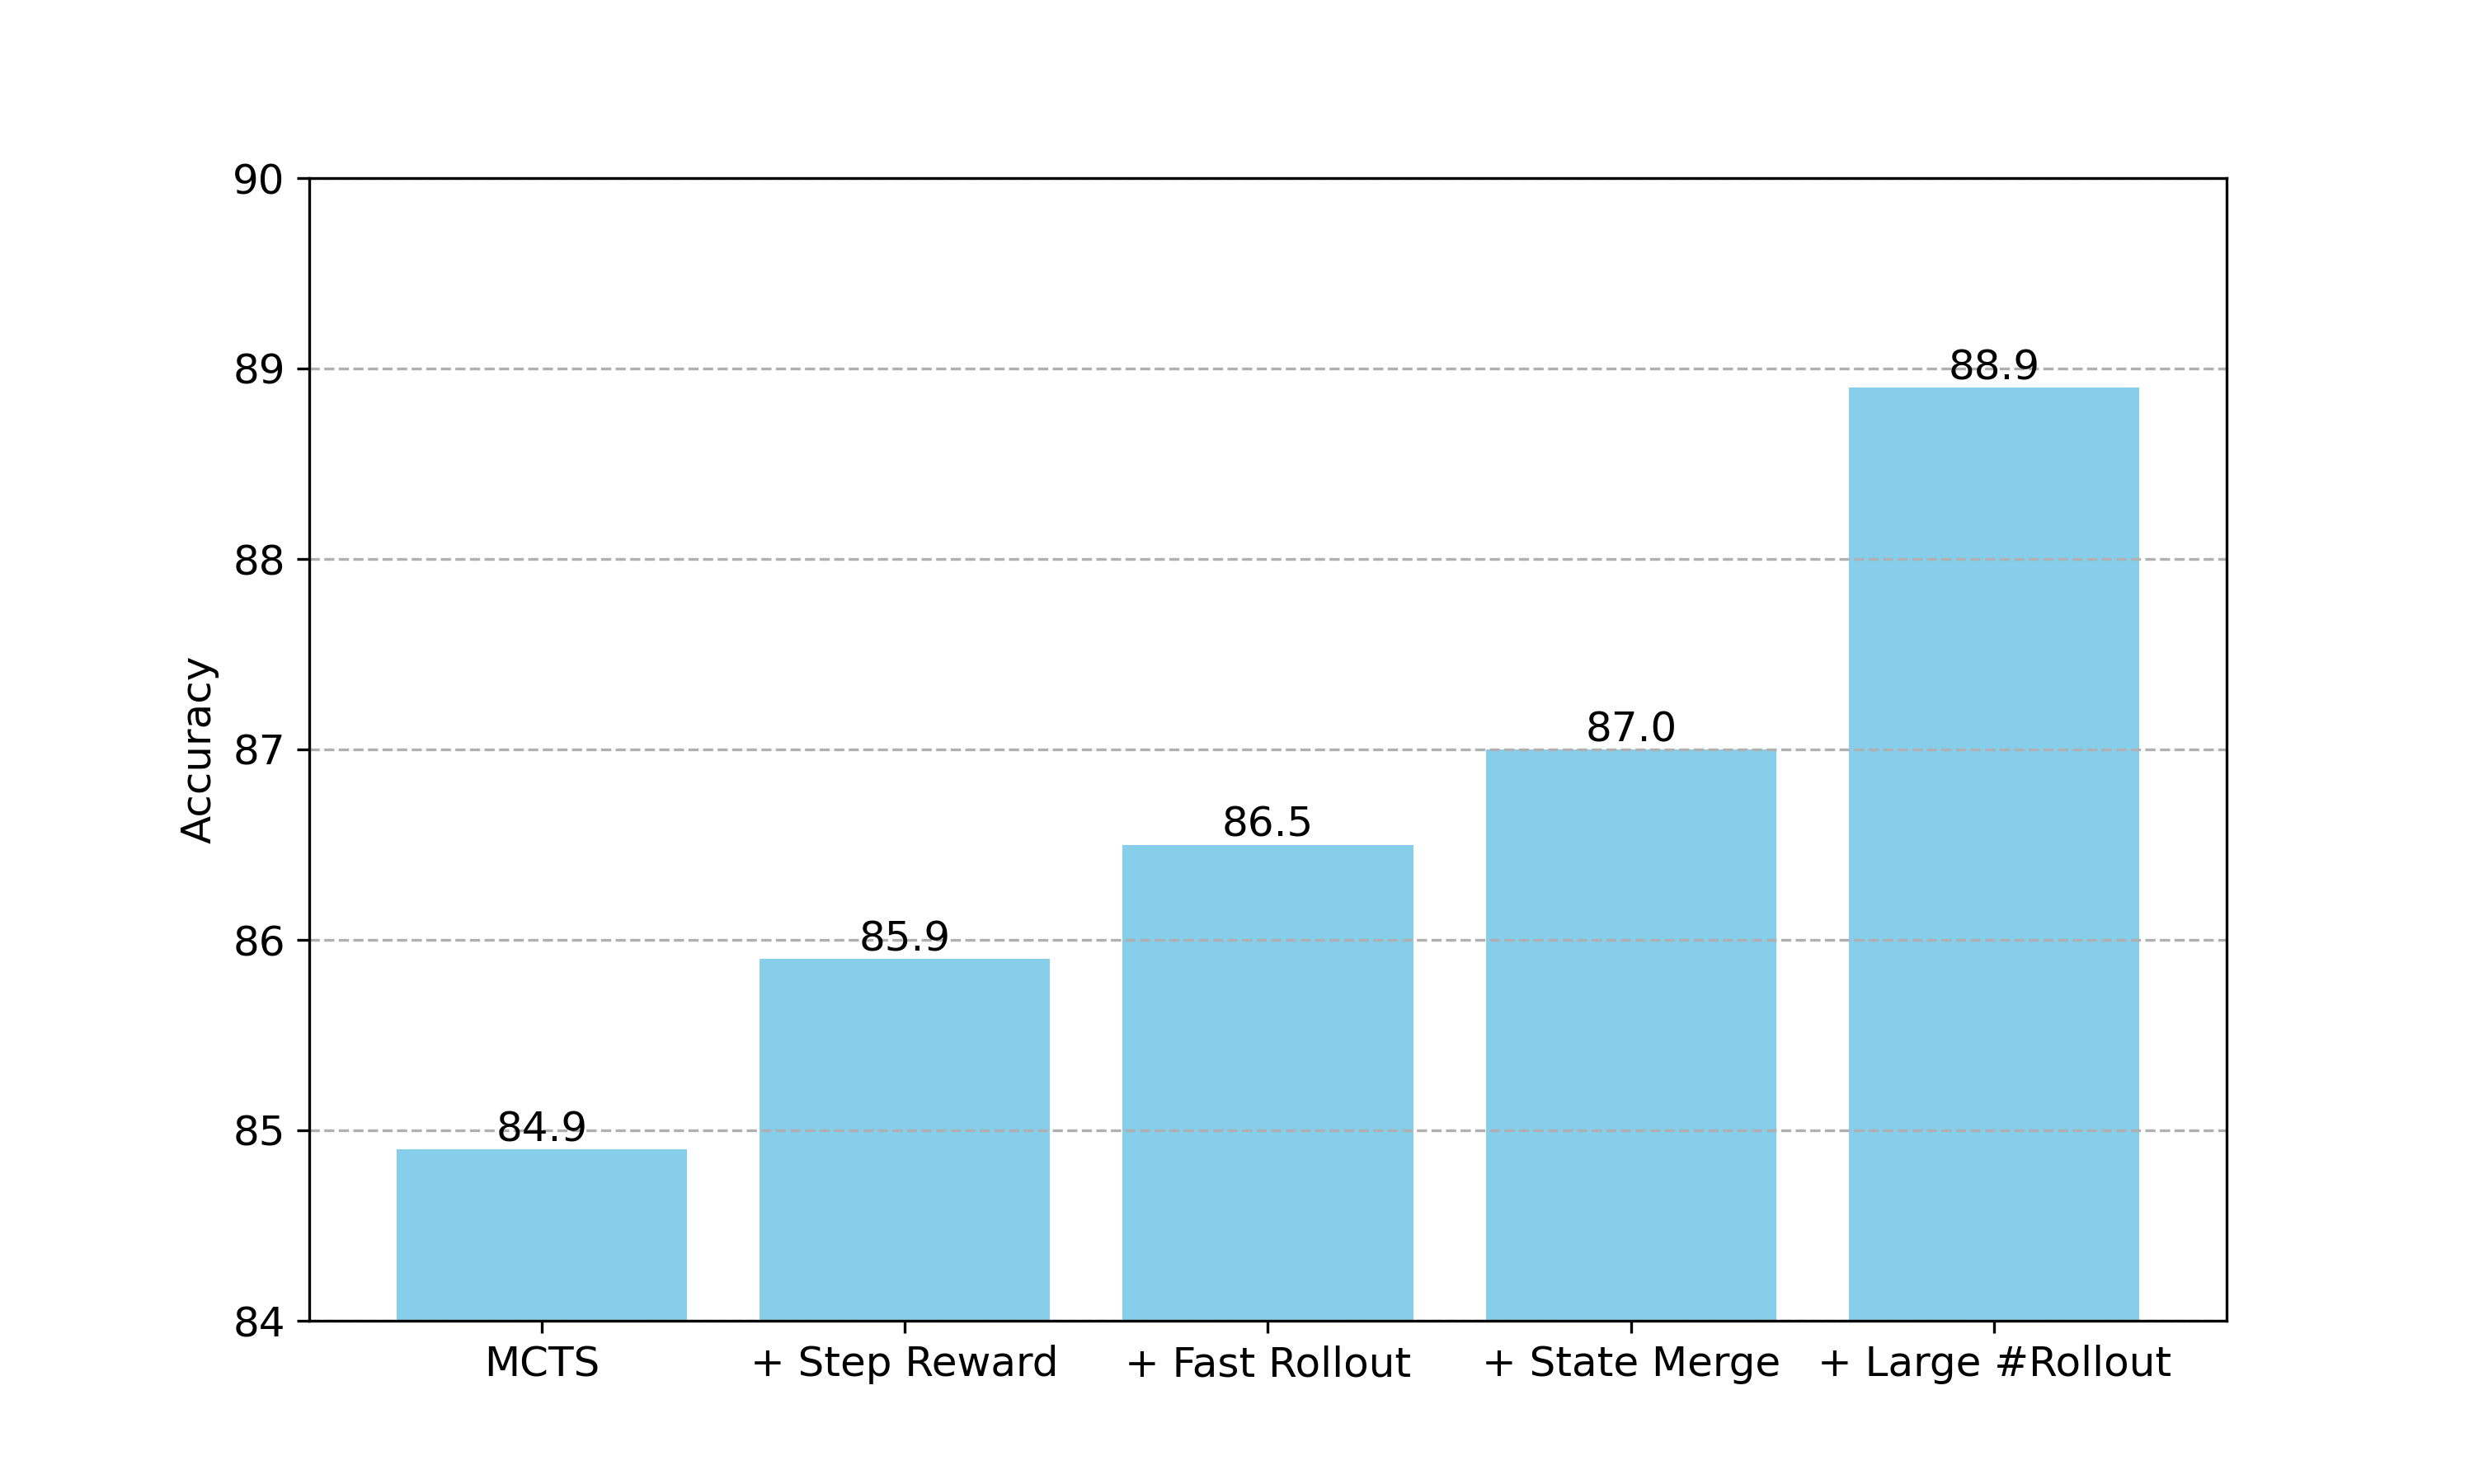
\includegraphics[width=0.75\textwidth]{figures/mcts_ablation.png}
    \caption{Ablation study on the GSM8K test set of various enhancements to the proposed efficient MCTS, including \prm{}, fastrollout with \orm{}, state merging, and increasing the number of rollouts.}
    \label{fig:search_ablation}
\end{figure}


% \begin{figure}[ht]
%     \centering
%     % Minipage for the Table
%     \begin{minipage}{0.25\textwidth}
%         \centering
%         \begin{tabular}{|l|c|}
%             \hline
%             Column 1 & Column 2 \\
%             \hline
%             Item 1 & Item 2 \\
%             Item 3 & Item 4 \\
%             \hline
%         \end{tabular}
%         \caption{Example Table}
%         \label{table:example_table}
%     \end{minipage}
%     \hfill
%     % Minipage for the Figure
%     \begin{minipage}{0.7\textwidth}
%         \centering
%         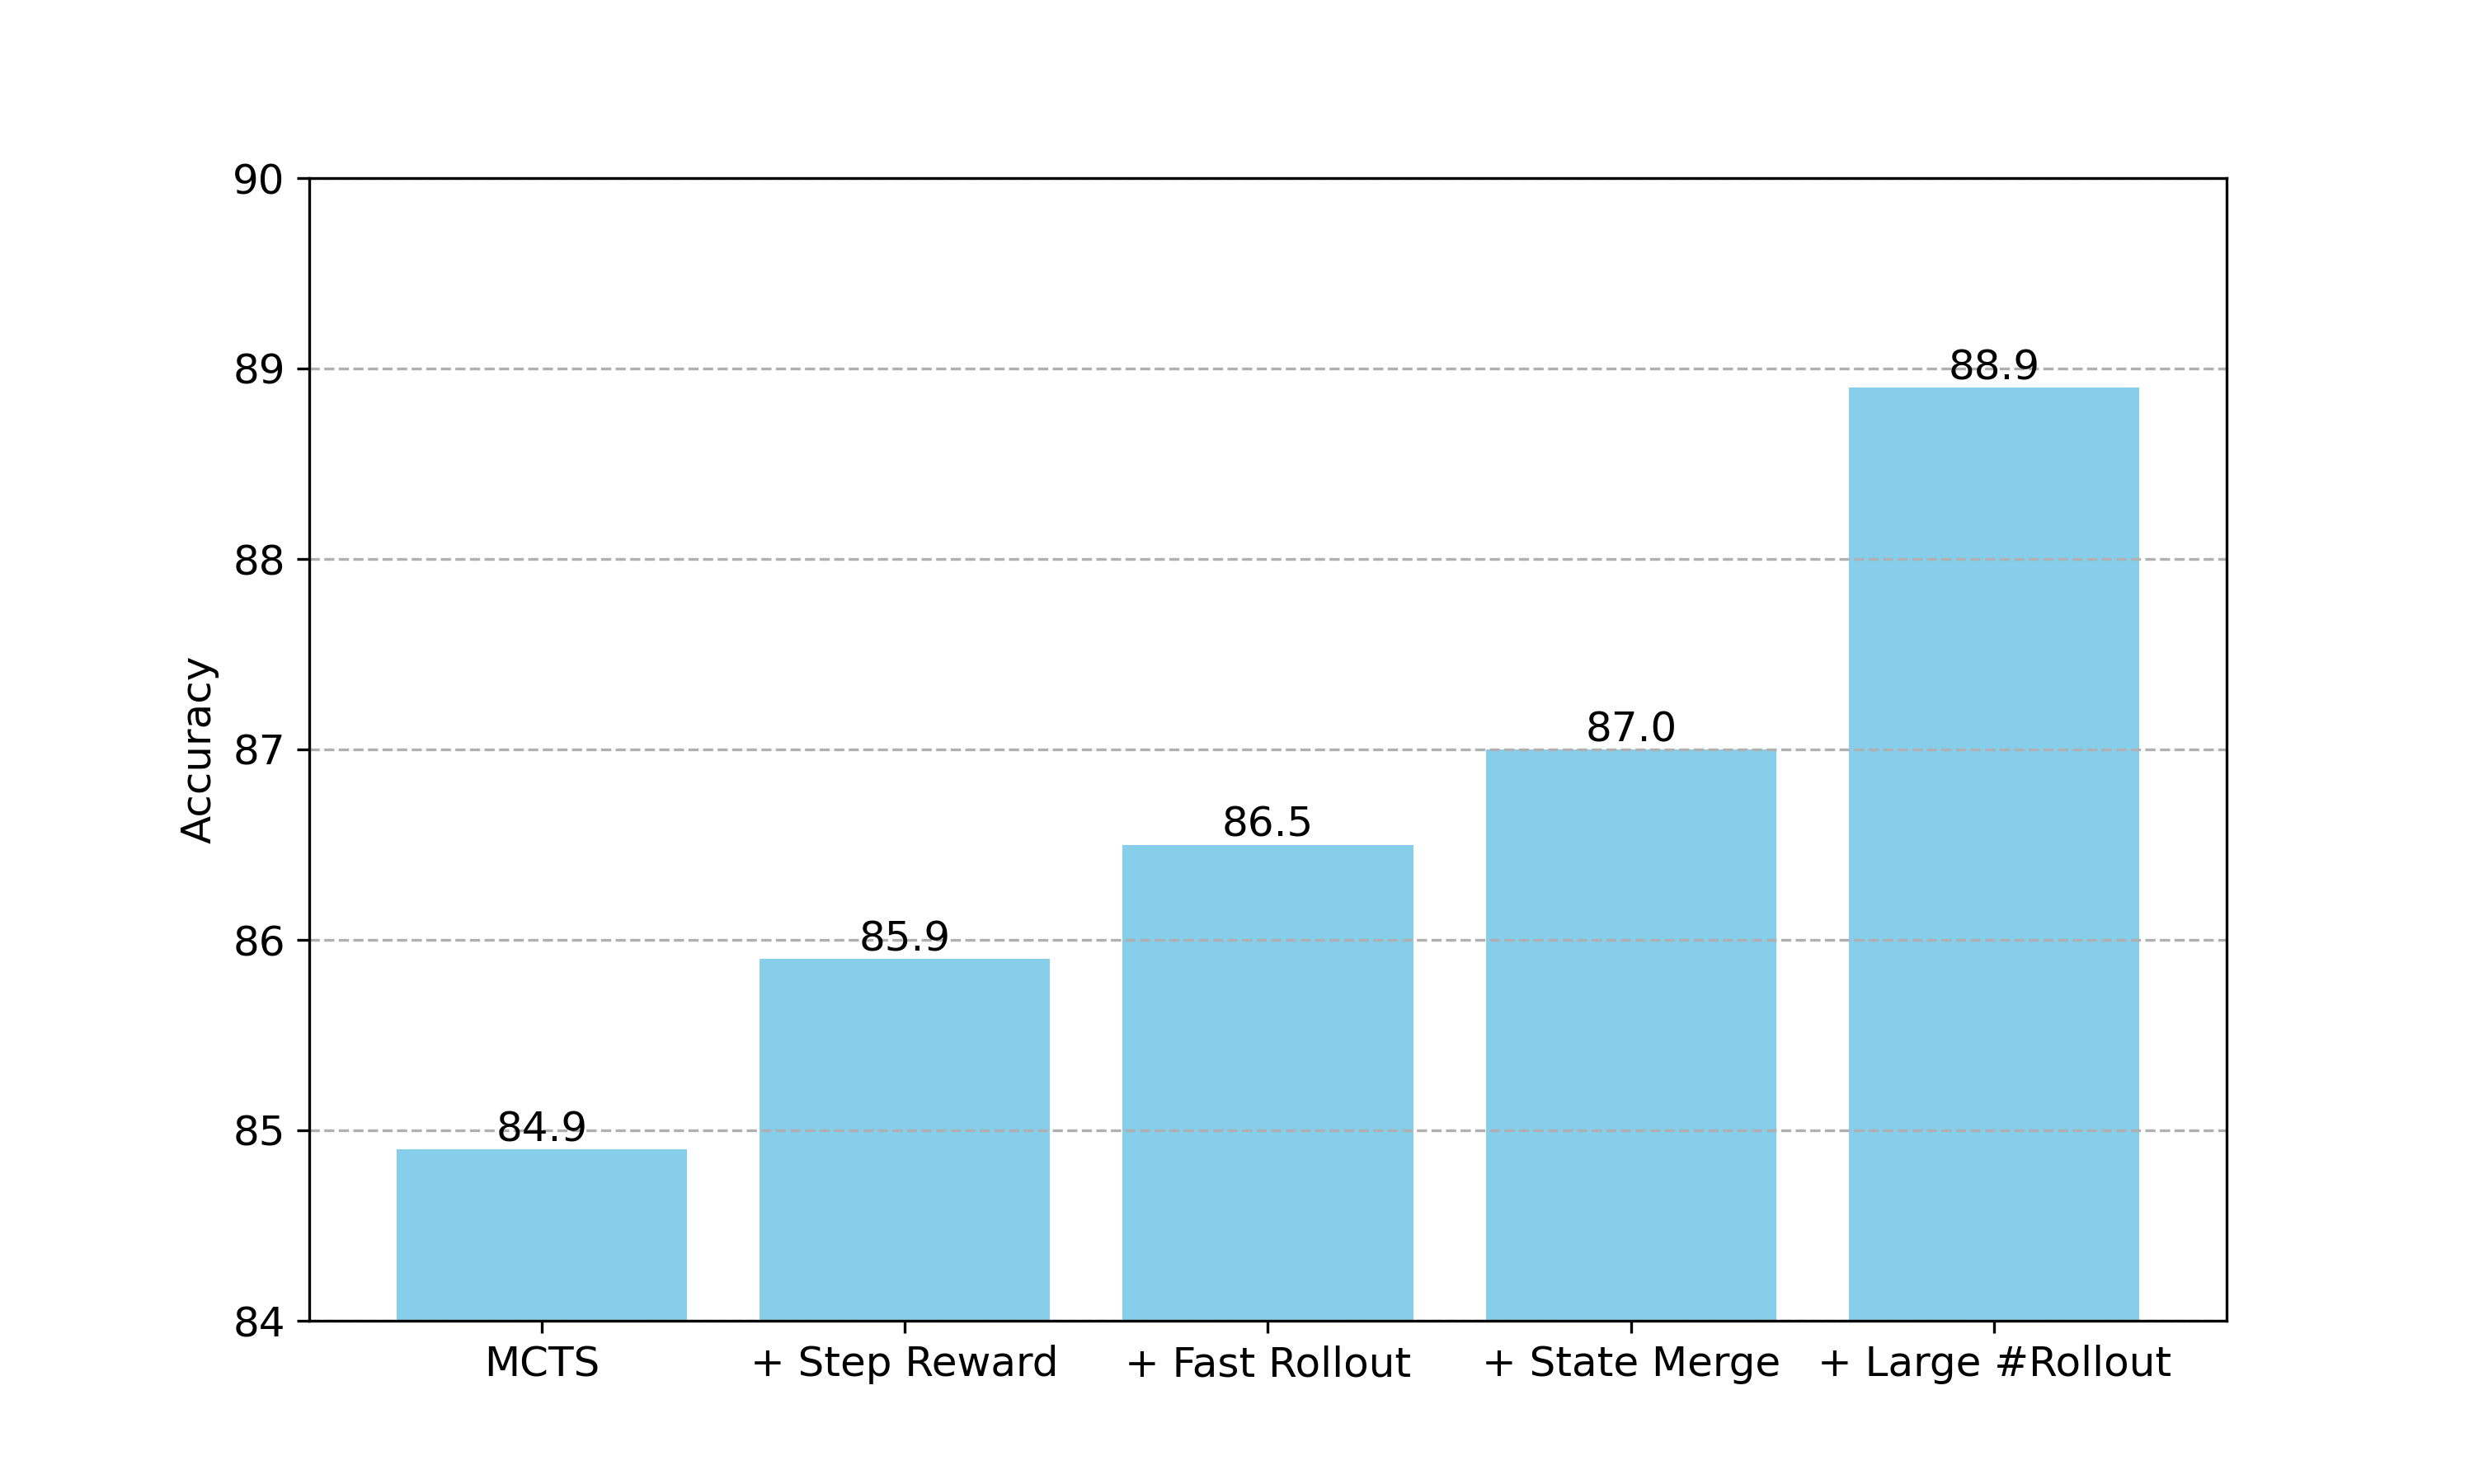
\includegraphics[width=0.9\textwidth]{figures/mcts_ablation.png}
%     \caption{Ablation study on the GSM8K test set of various enhancements to the proposed efficient MCTS, including \prm{}, fastrollout with \orm{}, state merging, and increasing the number of rollouts.}
%     \label{fig:search_ablation}
%     \end{minipage}
% \end{figure}

\begin{table}[h]
\small
\centering
\begin{minipage}{.5\linewidth}
\centering

\begin{tabular}{ccccc|c}
\toprule
\texttt{AB} & \prm{} & \texttt{FR}-\orm{} & \texttt{SM} & \texttt{LG-\#Rollout} & Acc \cr
\midrule
$\times$ & $\times$ & $\times$ & $\times$ & $\times$ & 79.5 \\
$\checkmark$ & $\times$ & $\times$ & $\times$ & $\times$ & 84.9 \\
$\checkmark$ & $\checkmark$ & $\times$ & $\times$ & $\times$ & 85.9 \\
$\checkmark$ & $\checkmark$ & $\checkmark$ & $\times$ & $\times$ & 86.5 \\
$\checkmark$ & $\checkmark$ & $\checkmark$ & $\checkmark$ & $\times$ & 87.0 \\
$\checkmark$ & $\checkmark$ & $\checkmark$ & $\checkmark$ & $\checkmark$ & 88.9 \\
\bottomrule
\end{tabular}
\vspace{2mm}
\caption*{(a) Ablation study on GSM8K}
% \caption{First Table: Ablation study on GSM8K test set.}
\end{minipage}%
\begin{minipage}{.5\linewidth}
\centering

\begin{tabular}{cc|cc}
\toprule
\texttt{TA}-\orm{} & \texttt{Option}  & \texttt{Acc} & \texttt{\#Rollout} \cr
\midrule
$\times$ & $\times$ & 38.8 & 201 \\
$\checkmark$ & $\times$ & 44.1 & 198 \\
$\checkmark$ & $\checkmark$ & 45.4 & 148 \\
\bottomrule
\end{tabular}
\vspace{2mm}
\caption*{(b) Ablation study on MATH}
\end{minipage}
\caption{\textbf{(a)}: Ablation studies on the GSM8K test set of various components of \emcts{}, including adaptive branching, \prm{}, fast-rollout with \orm{}, state merge, and large number of rollouts. \textbf{(b)}: Ablation studies of the impacts of tool-augmented \orm{} and option-level formulation  on MATH.}
\label{table:ablation}
\end{table}


We assess the effectiveness of each component in \model{} and report the results on GSM8K in Table~\ref{table:ablation}(a). Vanilla MCTS, configured with only the value function and a fixed number of children per node, achieves an accuracy of 79.5\%. This serves as a reference point for evaluating the incremental benefits introduced by each additional component. The use of adaptive branching increae the accuracy to 84.9\%. The addition of \prm{} improves the accuracy modestly to 85.9\%, showing the effectivenss of process supervision for searching. A more significant improvement is observed with the introduction of \orm{} with fast rollout, which boosts the accuracy to 86.5\%.  Integrating state merging results in a further increase in accuracy, reaching 87.0\%. Finally the combined of increasing the number of rollouts with the other components yields the best performance on this task. 

Table~\ref{table:ablation}(b) presents the ablation study of option formulation and the tool-augmented critic on the MATH dataset. Our proposed \emcts{} achieves an accuracy of 45.4 with 148 rollouts. When options are excluded, reverting to essentially sentence-level MCTS, the performance decreases to 44.1 with a noticeable increase in the number of rollouts to 198. This demonstrates that option formulation introduces enhanced flexibility to MCTS, enabling better performance with fewer search efforts. Furthermore, the most significant decrease in performance is observed when only intrinsic knowledge is utilized for \orm{}, which drops to an accuracy of 38.8. This suggests that the absence of an external tool critically impedes the \orm{}'s capability to effectively assess challenging math problems.


% \begin{wraptable}{r}{5.5cm}
% \label{tab:option_critic}
% % \vspace{-5mm}

% % \label{tab:my_label}
% \begin{tabular}{lcc}

% \toprule
% Method & \texttt{Acc} & \texttt{\#Rollout} \\
% \midrule
% \emcts{} & 45.4 & 148 \\
% \ w/o option & 44.1 & 198 \\
% \ \orm{} w/o tool  & 38.8 & 201 \\
% \bottomrule

% \end{tabular}
% \caption{Comparison results of options formulation on MATH.}
% \end{wraptable}
\begin{figure}[!tbp]
    \centering
    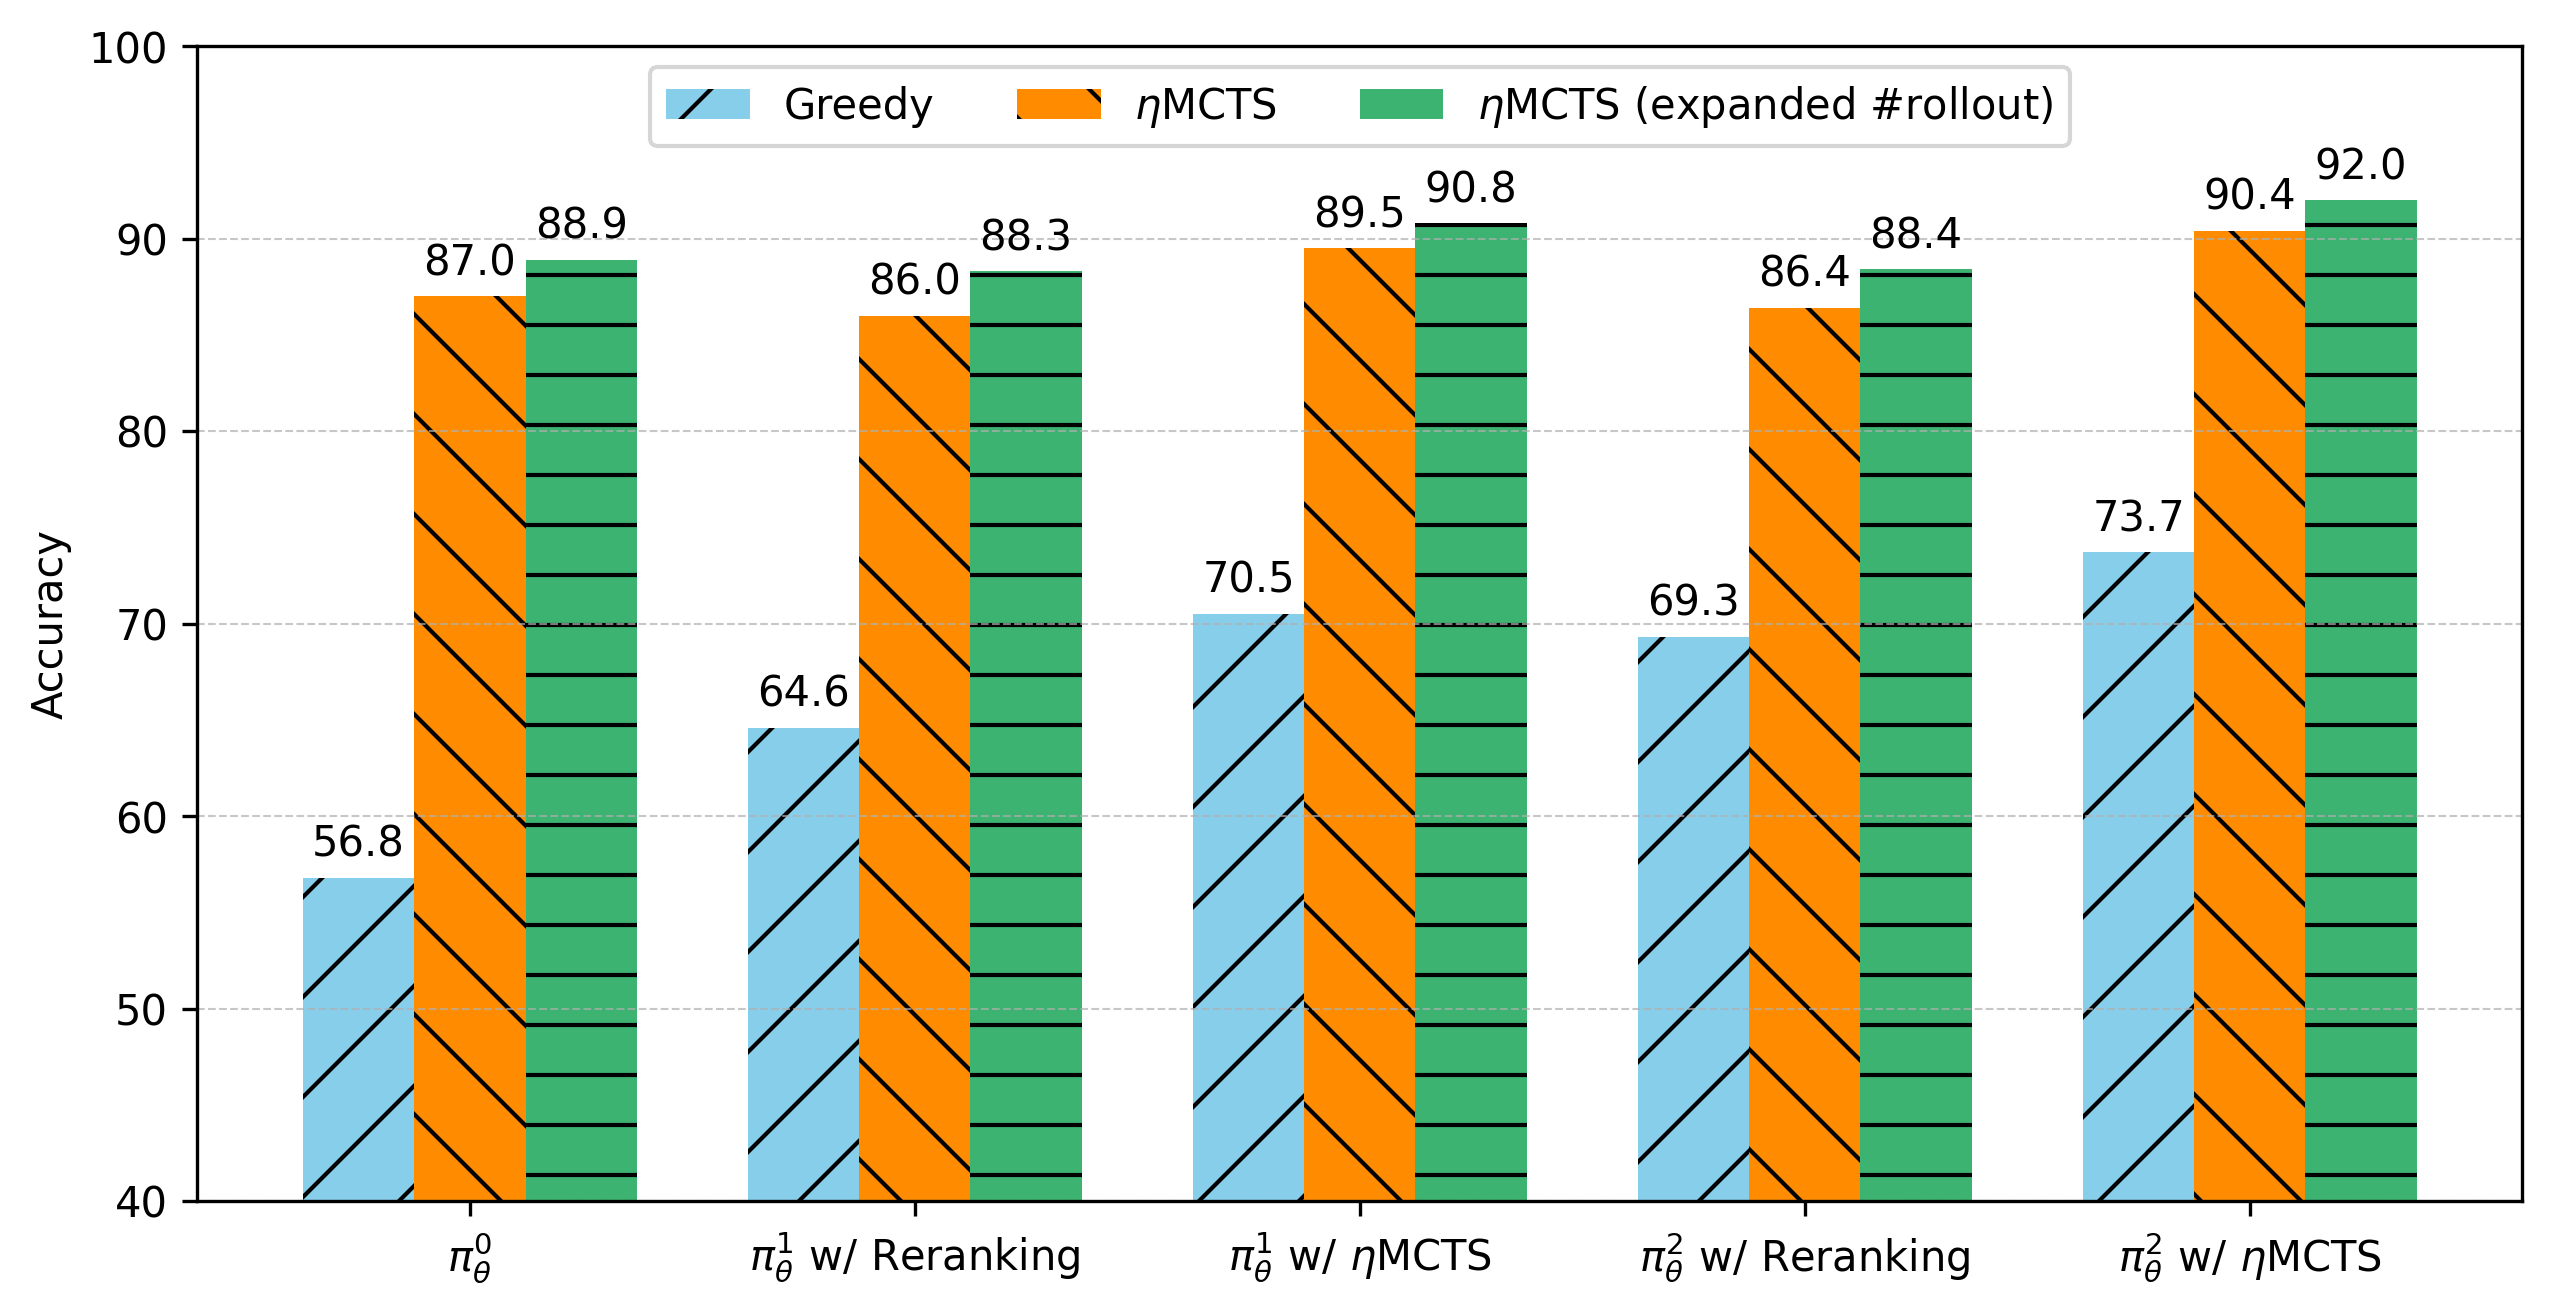
\includegraphics[width=0.9\textwidth]{figures/model_self_improving_n_rounds_results_v2.png}
    \caption{Empirical analysis on GSM8K of different self-improving data collection methods and number of iterations. Models are evaluated with greedy decoding, \emcts{} with small \#rollout and large \#rollout. }
    \label{fig:self_improving_ablations}
\end{figure}
Figure~\ref{fig:self_improving_ablations} depicts a comparative results on GSM8K of two rounds of self-improving trained on trajectories collected using reranking and \emcts{}. We report the performance of greedy decoding, \emcts{} with a relatively small number of rollouts (50-60), and \emcts{} with a larger number of rollouts (200-300) for each model. We observe that 1) Models trained on the trajectories from reranking or \emcts{} outperform the initial policy by a significant margin. In addition, the performance can be iteratively improved with training suggesting that self-improving has the potential to achieve continual performance gain. 2) While both reranking and \emcts{} can generate high-quality trajectories for self-improving , \emcts{} is performant with high efficiency and better accuracy. Models trained on trajectories generated by it not only exceed the performance of those trained on reranked trajectories but also, when decoded with \emcts{}, demonstrate on par performance with GPT-4, revealing that \model{} is an effective self-improving framework.

% 2) ablation study:
% search times, each components


\begin{table}[h]
\small
\centering
\begin{minipage}{.45\linewidth}
\centering

    \begin{tabular}{cl|c|c}
    \toprule
        \multicolumn{2}{c|}{\texttt{Method}}         & \texttt{Threshold}  & \texttt{Acc}\\
        % \hline
        \midrule
           &   Edit distance	               & $20$ & $86.8$ \\
           &   Edit distance	             & $50$ & $87.0$\\
           &  Cosine Similarity	            & $0.7$ & $86.3$\\
           & Model-based	& N/A	& $86.7$ \\
        \bottomrule
    \end{tabular}
\vspace{2mm}
\caption*{(a) Ablation on the choice of state merge functions.}
% \caption{First Table: Ablation study on GSM8K test set.}
\end{minipage}%
\begin{minipage}{.55\linewidth}
\centering

    \begin{tabular}{cl|c}
    \toprule
        \multicolumn{2}{c|}{\texttt{\#Trajetory}}         & \texttt{Acc}\\
        \midrule
           &   $1$	                & $85.9$ \\
           &   $4$	           & $86.5$\\
           &  $8$	       & $86.7$\\
        \bottomrule
    \end{tabular}
\vspace{2mm}
\caption*{(b) Ablation on the number of trajectories.}
\end{minipage}
\caption{\textbf{(a)}: Ablation studies on the choice of heuristic/model-based functions in state merge on GSM8K with base Llama2-70b. The model used in the model-based state merge is Llama-2-70b-chat. \textbf{(b)}: Ablation studies of the number of rollout trajectories in fast-rollout estimation on GSM8K with base Llama2-70b.}
\label{table:ablation_sm}
\end{table}

We further analyze the impact of different hyperparameters and design choices for each component. Table~\ref{table:ablation_sm}(a) shows that varying heuristic functions (with hyperparameters) for state merge has limited impact on performance. Table~\ref{table:ablation_sm}(b) shows that, as the number of fast-rollouts increases, there is a corresponding improvement in performance. This is due to the reduction in the variance of the estimates. We used $n=4$ in our experiments for better trade-off between performance and efficiency. Additional ablations on the choice of fast-rollout models, are provided in Appendix \ref{app:add_ablations}.


% Analysis: 
% x: bin of acc.  y: avg step/outcome reward
% value acc. for fast-rollout vs no fast-rollout
% Tool use vs. no tool use on MATH set (v$_2$ small vs. v$_4$ small)

% \subsection{Self-improving Results}





% % \section{Limitations and Future Work}
% % Despite the promising results demonstrated by \model{} in this study, there are several limitations that requires further exploration. (\RN{1}) Our current implementation employs relatively simple methods for generating synthetic prompts. Future iterations of \model{} should explore advanced techniques, such as Self-Instruct, to create both diverse and model capability-awared prompts. (\RN{2}) Although \model{} demonstrates improvements over base models, its performance in greedy sampling is substantially inferior to that observed when decoded with \emcts{}. This indicates that the full potential of MCTS for self-improvement in LLMs has not yet been fully realized. Two potential factors contributing to this issue have been identified: a) the self-improvement loop may not be leveraging sufficient data; and b) the base model may be limited in its capacity for rapid learning. Addressing these concerns could lead to more significant improvemens. (\RN{3}) In our existing framework, the critic models remain static. We will explore mechanisms to continually update critic models to adapt to new policy models. This will help ensure the discriminator-generator gap and improve the overall training dynamics. (\RN{4}) The evaluation of \model{} has been limited to mathematical reasoning tasks. To verify the generalizability and broader applicability of the framework, future research will need to extend its application to other domains.

% \section{Conclusion}
% \label{sec:con}
% In this paper, we introduce \model{}, an imagination-searching-criticizing framework designed for the self-improvement of LLMs without the necessity of additional annotations. At the heart of it is the integration of MCTS with LLMs. To tackle the inherent challenges associated with this integration, including data scarcity, the vastness of search spaces, and the subjective nature of feedback in language tasks, we introduce a data synthesizer for strategic prompt synthesis, an optimized MCTS tailored for efficient search in language tasks, and a trio of critic models to provide precise feedback. Our experimental findings on mathematical reasoning tasks reveal that \model{} significantly boosts the performance of LLMs without requiring extra data annotations. Moreover, when decoded with \emcts{}, \model{} performs comparably to GPT-4, highlighting the potential for self-improvement in LLMs.

% \section{Limitations}
% \label{sec:limitations}

% \medskip
% \newpage
% \bibliography{neurips_2023}
% \bibliographystyle{iclr2021_conference}

\end{document}